\documentclass[twoside]{book}

% Packages required by doxygen
\usepackage{fixltx2e}
\usepackage{calc}
\usepackage{doxygen}
\usepackage[export]{adjustbox} % also loads graphicx
\usepackage{graphicx}
\usepackage[utf8]{inputenc}
\usepackage{makeidx}
\usepackage{multicol}
\usepackage{multirow}
\PassOptionsToPackage{warn}{textcomp}
\usepackage{textcomp}
\usepackage[nointegrals]{wasysym}
\usepackage[table]{xcolor}

% Font selection
\usepackage[T1]{fontenc}
\usepackage[scaled=.90]{helvet}
\usepackage{courier}
\usepackage{amssymb}
\usepackage{sectsty}
\renewcommand{\familydefault}{\sfdefault}
\allsectionsfont{%
  \fontseries{bc}\selectfont%
  \color{darkgray}%
}
\renewcommand{\DoxyLabelFont}{%
  \fontseries{bc}\selectfont%
  \color{darkgray}%
}
\newcommand{\+}{\discretionary{\mbox{\scriptsize$\hookleftarrow$}}{}{}}

% Page & text layout
\usepackage{geometry}
\geometry{%
  a4paper,%
  top=2.5cm,%
  bottom=2.5cm,%
  left=2.5cm,%
  right=2.5cm%
}
\tolerance=750
\hfuzz=15pt
\hbadness=750
\setlength{\emergencystretch}{15pt}
\setlength{\parindent}{0cm}
\setlength{\parskip}{3ex plus 2ex minus 2ex}
\makeatletter
\renewcommand{\paragraph}{%
  \@startsection{paragraph}{4}{0ex}{-1.0ex}{1.0ex}{%
    \normalfont\normalsize\bfseries\SS@parafont%
  }%
}
\renewcommand{\subparagraph}{%
  \@startsection{subparagraph}{5}{0ex}{-1.0ex}{1.0ex}{%
    \normalfont\normalsize\bfseries\SS@subparafont%
  }%
}
\makeatother

% Headers & footers
\usepackage{fancyhdr}
\pagestyle{fancyplain}
\fancyhead[LE]{\fancyplain{}{\bfseries\thepage}}
\fancyhead[CE]{\fancyplain{}{}}
\fancyhead[RE]{\fancyplain{}{\bfseries\leftmark}}
\fancyhead[LO]{\fancyplain{}{\bfseries\rightmark}}
\fancyhead[CO]{\fancyplain{}{}}
\fancyhead[RO]{\fancyplain{}{\bfseries\thepage}}
\fancyfoot[LE]{\fancyplain{}{}}
\fancyfoot[CE]{\fancyplain{}{}}
\fancyfoot[RE]{\fancyplain{}{\bfseries\scriptsize Generated by Doxygen }}
\fancyfoot[LO]{\fancyplain{}{\bfseries\scriptsize Generated by Doxygen }}
\fancyfoot[CO]{\fancyplain{}{}}
\fancyfoot[RO]{\fancyplain{}{}}
\renewcommand{\footrulewidth}{0.4pt}
\renewcommand{\chaptermark}[1]{%
  \markboth{#1}{}%
}
\renewcommand{\sectionmark}[1]{%
  \markright{\thesection\ #1}%
}

% Indices & bibliography
\usepackage{natbib}
\usepackage[titles]{tocloft}
\setcounter{tocdepth}{3}
\setcounter{secnumdepth}{5}
\makeindex

% Hyperlinks (required, but should be loaded last)
\usepackage{ifpdf}
\ifpdf
  \usepackage[pdftex,pagebackref=true]{hyperref}
\else
  \usepackage[ps2pdf,pagebackref=true]{hyperref}
\fi
\hypersetup{%
  colorlinks=true,%
  linkcolor=blue,%
  citecolor=blue,%
  unicode%
}

% Custom commands
\newcommand{\clearemptydoublepage}{%
  \newpage{\pagestyle{empty}\cleardoublepage}%
}

\usepackage{caption}
\captionsetup{labelsep=space,justification=centering,font={bf},singlelinecheck=off,skip=4pt,position=top}

%===== C O N T E N T S =====

\begin{document}

% Titlepage & ToC
\hypersetup{pageanchor=false,
             bookmarksnumbered=true,
             pdfencoding=unicode
            }
\pagenumbering{alph}
\begin{titlepage}
\vspace*{7cm}
\begin{center}%
{\Large Uniform Data Operator \\[1ex]\large 0.\+1 }\\
\vspace*{1cm}
{\large Generated by Doxygen 1.8.14}\\
\end{center}
\end{titlepage}
\clearemptydoublepage
\pagenumbering{roman}
\tableofcontents
\clearemptydoublepage
\pagenumbering{arabic}
\hypersetup{pageanchor=true}

%--- Begin generated contents ---
\chapter{Uniform Data Operator}
\label{md__d_1__work__git_hub_uniform-data-operator__readme}
\Hypertarget{md__d_1__work__git_hub_uniform-data-operator__readme}
It\textquotesingle{}s a framework that allow to oparate and manage yours data by unified way, not depending from your data base or prefered format. Standardize your data structures and avoid tuning of your product only for one storage type that could be not suitable for you in future.

\section*{Modules}

\subsection*{Binnary Handler}

Provides base A\+PI for binary serizliation process.

\subsection*{S\+Q\+L\+Operator\+Handler}

Provides methods that simplify comnverting app data to query format. Inform subscribers about S\+QL operators events. Provides access to current Active S\+QL operator.

\subsection*{Attributes\+Handler}

Provides A\+PI thats simplify working with U\+DO attributes and members data.

\subsection*{Included operators\+:}


\begin{DoxyItemize}
\item My\+S\+Q\+L\+Data\+Operator -\/ provides uniform way to manage your data via My\+S\+QL database.
\end{DoxyItemize}

\section*{F.\+A.\+Q.}

\subsection*{How to describe table class/struct?}

\subsubsection*{Conception}

At first you need to understand conception of work with data and them representations at database.

For every table on server that must be compatible with your application on native level you need to provide the class/structure with compatible and correct described fields/properties.

This class/structure would be a bridge betwee your local data and server representation.

\subsubsection*{Describing}

Describing of data making by using of attributs from \textquotesingle{}\mbox{\hyperlink{namespace_uniform_data_operator_1_1_sql_1_1_tables_1_1_attributes}{Uniform\+Data\+Operator.\+Sql.\+Tables.\+Attributes}}\textquotesingle{} namespace. (Custom attributes and modifiers can has other namespace).


\begin{DoxyEnumerate}
\item Define \textquotesingle{}Table\textquotesingle{} attribute for your class/structure. Describe correct scheme and table name.
\item Define \textquotesingle{}System.\+Serializable\textquotesingle{} attribute for your class.
\item For every field/property that would be a column defind \textquotesingle{}Column\textquotesingle{} attribute. Set column name and type at constructor.
\item Define additive columns\textquotesingle{} attributes like \textquotesingle{}is\+Primary\+Key\textquotesingle{}, \textquotesingle{}is\+Auto\+Increment\textquotesingle{}, \textquotesingle{}Commentary\textquotesingle{}, etc. More details you can wind in source or offline documetation.
\end{DoxyEnumerate}

\subsection*{How operator defines what would be included in auto generated read/write queries?}

Every operator can has a different algorithm related to specific requirements of database server. But a common idea is mapping of you \textquotesingle{}Table\textquotesingle{} defined class by \textquotesingle{}Column\textquotesingle{} attributes and generate the queries based on them settings and values.

If some attribute affecting algorithm then that described at that\textquotesingle{}s summary.

\subsection*{I need to manage data received from server. How I can do it?}

Just use the property as column. Then you would be able to manage a complex get/set algorithms during operator actions.

\subsection*{Can I add supporting of other S\+QL server?}

Sure. Just create you Server\+Nam\+Operator that implement I\+Sql\+Operator interface and your data described by U\+DO\textquotesingle{}s attributes would be compatible with your specific server.

Use the default My\+Sql\+Data\+Operator (group of partial classes) as example. Them are pretty good documented. If you done this job please consider sharing this source as contribution into U\+DO.

\subsection*{My S\+QL server incompatible with Db\+Data\+Type\textquotesingle{}s indexes. How I can adjust my data?}

By default \textquotesingle{}Column\textquotesingle{} attribute described via Db\+Data\+Type that mostly unusable for huge count of types that custom for every different S\+QL server. If you faced with such kind of problem so just create your own modifying attribute that would be used on your custom I\+Sql\+Operator instance.

Use \textquotesingle{}\mbox{\hyperlink{class_uniform_data_operator_1_1_sql_1_1_my_sql_1_1_attributes_1_1_my_sql_d_b_type_override}{Uniform\+Data\+Operator.\+Sql.\+My\+Sql.\+Attributes.\+My\+Sql\+D\+B\+Type\+Override}}\textquotesingle{} as example for your source. Check how it using at \textquotesingle{}My\+Sql\+Data\+Operator\+Commands.\+cs\textquotesingle{} in \textquotesingle{}Column\+Declaration\+Command\textquotesingle{} method.

\subsection*{Auto write/read not enough flexible for me. How I can make custom query?}

Auto managing of duplex exchanging of data with S\+QL server it\textquotesingle{}s just a high end feature. But not the only way to manage your data by uniformed way.

All what you need it\textquotesingle{}s pipe down on one level and start direct work with your \textquotesingle{}I\+Sql\+Operator\textquotesingle{} instance.

Make your own S\+QL query suitable by your specific task and send it to server via \textquotesingle{}Sql\+Operato\+Handler.\+Active\textquotesingle{} by use one of provided methods \+:
\begin{DoxyItemize}
\item \textquotesingle{}Execute\+Non\+Query\textquotesingle{}
\item \textquotesingle{}Execute\+Scalar\textquotesingle{}
\item \textquotesingle{}Execute\+Reader\textquotesingle{}
\item \textquotesingle{}Count\textquotesingle{}
\end{DoxyItemize}

\subsection*{How to establish connection with server?}


\begin{DoxyEnumerate}
\item Create and instance of your \textquotesingle{}I\+Sql\+Operator\textquotesingle{}.
\item Initialize properties of your \textquotesingle{}I\+Sql\+Operator\textquotesingle{}\+:
\begin{DoxyItemize}
\item string Server
\item int Port
\item string Database
\item string User\+Id
\item string Password
\end{DoxyItemize}
\item Call \textquotesingle{}Inialize\textquotesingle{} method on your \textquotesingle{}I\+Sql\+Operator\textquotesingle{}.
\item Call \textquotesingle{}Open\+Connection\textquotesingle{} method on your \textquotesingle{}I\+Sql\+Operator\textquotesingle{}.
\item Execute your Sql query.
\item Call \textquotesingle{}Close\+Connection\textquotesingle{} method on your \textquotesingle{}I\+Sql\+Operator\textquotesingle{} 
\end{DoxyEnumerate}
\chapter{Namespace Index}
\section{Packages}
Here are the packages with brief descriptions (if available)\+:\begin{DoxyCompactList}
\item\contentsline{section}{\mbox{\hyperlink{namespace_base_tests}{Base\+Tests}} }{\pageref{namespace_base_tests}}{}
\item\contentsline{section}{\mbox{\hyperlink{namespace_base_tests_1_1_binary}{Base\+Tests.\+Binary}} }{\pageref{namespace_base_tests_1_1_binary}}{}
\item\contentsline{section}{\mbox{\hyperlink{namespace_base_tests_1_1_types}{Base\+Tests.\+Types}} }{\pageref{namespace_base_tests_1_1_types}}{}
\item\contentsline{section}{\mbox{\hyperlink{namespace_my_s_q_l_tests}{My\+S\+Q\+L\+Tests}} }{\pageref{namespace_my_s_q_l_tests}}{}
\item\contentsline{section}{\mbox{\hyperlink{namespace_uniform_data_operator}{Uniform\+Data\+Operator}} }{\pageref{namespace_uniform_data_operator}}{}
\item\contentsline{section}{\mbox{\hyperlink{namespace_uniform_data_operator_1_1_binary}{Uniform\+Data\+Operator.\+Binary}} }{\pageref{namespace_uniform_data_operator_1_1_binary}}{}
\item\contentsline{section}{\mbox{\hyperlink{namespace_uniform_data_operator_1_1_sql}{Uniform\+Data\+Operator.\+Sql}} }{\pageref{namespace_uniform_data_operator_1_1_sql}}{}
\item\contentsline{section}{\mbox{\hyperlink{namespace_uniform_data_operator_1_1_sql_1_1_attributes}{Uniform\+Data\+Operator.\+Sql.\+Attributes}} }{\pageref{namespace_uniform_data_operator_1_1_sql_1_1_attributes}}{}
\item\contentsline{section}{\mbox{\hyperlink{namespace_uniform_data_operator_1_1_sql_1_1_attributes_1_1_modifiers}{Uniform\+Data\+Operator.\+Sql.\+Attributes.\+Modifiers}} }{\pageref{namespace_uniform_data_operator_1_1_sql_1_1_attributes_1_1_modifiers}}{}
\item\contentsline{section}{\mbox{\hyperlink{namespace_uniform_data_operator_1_1_sql_1_1_my_sql}{Uniform\+Data\+Operator.\+Sql.\+My\+Sql}} }{\pageref{namespace_uniform_data_operator_1_1_sql_1_1_my_sql}}{}
\item\contentsline{section}{\mbox{\hyperlink{namespace_uniform_data_operator_1_1_sql_1_1_my_sql_1_1_attributes}{Uniform\+Data\+Operator.\+Sql.\+My\+Sql.\+Attributes}} }{\pageref{namespace_uniform_data_operator_1_1_sql_1_1_my_sql_1_1_attributes}}{}
\end{DoxyCompactList}

\chapter{Hierarchical Index}
\section{Class Hierarchy}
This inheritance list is sorted roughly, but not completely, alphabetically\+:\begin{DoxyCompactList}
\item Attribute\begin{DoxyCompactList}
\item \contentsline{section}{Uniform\+Data\+Operator.\+Sql.\+My\+Sql.\+Attributes.\+My\+Sql\+D\+B\+Type\+Override}{\pageref{class_uniform_data_operator_1_1_sql_1_1_my_sql_1_1_attributes_1_1_my_sql_d_b_type_override}}{}
\item \contentsline{section}{Uniform\+Data\+Operator.\+Sql.\+Tables.\+Attributes.\+Column}{\pageref{class_uniform_data_operator_1_1_sql_1_1_tables_1_1_attributes_1_1_column}}{}
\item \contentsline{section}{Uniform\+Data\+Operator.\+Sql.\+Tables.\+Attributes.\+Commentary}{\pageref{class_uniform_data_operator_1_1_sql_1_1_tables_1_1_attributes_1_1_commentary}}{}
\item \contentsline{section}{Uniform\+Data\+Operator.\+Sql.\+Tables.\+Attributes.\+Default}{\pageref{class_uniform_data_operator_1_1_sql_1_1_tables_1_1_attributes_1_1_default}}{}
\begin{DoxyCompactList}
\item \contentsline{section}{Uniform\+Data\+Operator.\+Sql.\+Tables.\+Attributes.\+Is\+Generated}{\pageref{class_uniform_data_operator_1_1_sql_1_1_tables_1_1_attributes_1_1_is_generated}}{}
\end{DoxyCompactList}
\item \contentsline{section}{Uniform\+Data\+Operator.\+Sql.\+Tables.\+Attributes.\+Is\+Auto\+Increment}{\pageref{class_uniform_data_operator_1_1_sql_1_1_tables_1_1_attributes_1_1_is_auto_increment}}{}
\item \contentsline{section}{Uniform\+Data\+Operator.\+Sql.\+Tables.\+Attributes.\+Is\+Binary}{\pageref{class_uniform_data_operator_1_1_sql_1_1_tables_1_1_attributes_1_1_is_binary}}{}
\item \contentsline{section}{Uniform\+Data\+Operator.\+Sql.\+Tables.\+Attributes.\+Is\+Foreign\+Key}{\pageref{class_uniform_data_operator_1_1_sql_1_1_tables_1_1_attributes_1_1_is_foreign_key}}{}
\item \contentsline{section}{Uniform\+Data\+Operator.\+Sql.\+Tables.\+Attributes.\+Is\+Not\+Null}{\pageref{class_uniform_data_operator_1_1_sql_1_1_tables_1_1_attributes_1_1_is_not_null}}{}
\item \contentsline{section}{Uniform\+Data\+Operator.\+Sql.\+Tables.\+Attributes.\+Is\+Primary\+Key}{\pageref{class_uniform_data_operator_1_1_sql_1_1_tables_1_1_attributes_1_1_is_primary_key}}{}
\item \contentsline{section}{Uniform\+Data\+Operator.\+Sql.\+Tables.\+Attributes.\+Is\+Unique}{\pageref{class_uniform_data_operator_1_1_sql_1_1_tables_1_1_attributes_1_1_is_unique}}{}
\item \contentsline{section}{Uniform\+Data\+Operator.\+Sql.\+Tables.\+Attributes.\+Is\+Unsigned}{\pageref{class_uniform_data_operator_1_1_sql_1_1_tables_1_1_attributes_1_1_is_unsigned}}{}
\item \contentsline{section}{Uniform\+Data\+Operator.\+Sql.\+Tables.\+Attributes.\+Is\+Zero\+Fill}{\pageref{class_uniform_data_operator_1_1_sql_1_1_tables_1_1_attributes_1_1_is_zero_fill}}{}
\item \contentsline{section}{Uniform\+Data\+Operator.\+Sql.\+Tables.\+Attributes.\+Modifiers.\+Set\+Query\+Ignore}{\pageref{class_uniform_data_operator_1_1_sql_1_1_tables_1_1_attributes_1_1_modifiers_1_1_set_query_ignore}}{}
\item \contentsline{section}{Uniform\+Data\+Operator.\+Sql.\+Tables.\+Attributes.\+Table}{\pageref{class_uniform_data_operator_1_1_sql_1_1_tables_1_1_attributes_1_1_table}}{}
\end{DoxyCompactList}
\item \contentsline{section}{Uniform\+Data\+Operator.\+Attributes\+Handler}{\pageref{class_uniform_data_operator_1_1_attributes_handler}}{}
\item \contentsline{section}{Uniform\+Data\+Operator.\+Binary.\+Binary\+Handler}{\pageref{class_uniform_data_operator_1_1_binary_1_1_binary_handler}}{}
\item \contentsline{section}{Base\+Tests.\+Binary.\+Binary\+Handler\+Tests}{\pageref{class_base_tests_1_1_binary_1_1_binary_handler_tests}}{}
\item \contentsline{section}{Base\+Tests.\+Types.\+Blob\+Type}{\pageref{class_base_tests_1_1_types_1_1_blob_type}}{}
\item \contentsline{section}{Uniform\+Data\+Operator.\+Sql.\+I\+Sql\+Operator}{\pageref{interface_uniform_data_operator_1_1_sql_1_1_i_sql_operator}}{}
\begin{DoxyCompactList}
\item \contentsline{section}{Uniform\+Data\+Operator.\+Sql.\+My\+Sql.\+My\+Sql\+Data\+Operator}{\pageref{class_uniform_data_operator_1_1_sql_1_1_my_sql_1_1_my_sql_data_operator}}{}
\item \contentsline{section}{Uniform\+Data\+Operator.\+Sql.\+My\+Sql.\+My\+Sql\+Data\+Operator}{\pageref{class_uniform_data_operator_1_1_sql_1_1_my_sql_1_1_my_sql_data_operator}}{}
\item \contentsline{section}{Uniform\+Data\+Operator.\+Sql.\+My\+Sql.\+My\+Sql\+Data\+Operator}{\pageref{class_uniform_data_operator_1_1_sql_1_1_my_sql_1_1_my_sql_data_operator}}{}
\item \contentsline{section}{Uniform\+Data\+Operator.\+Sql.\+My\+Sql.\+My\+Sql\+Data\+Operator}{\pageref{class_uniform_data_operator_1_1_sql_1_1_my_sql_1_1_my_sql_data_operator}}{}
\item \contentsline{section}{Uniform\+Data\+Operator.\+Sql.\+My\+Sql.\+My\+Sql\+Data\+Operator}{\pageref{class_uniform_data_operator_1_1_sql_1_1_my_sql_1_1_my_sql_data_operator}}{}
\item \contentsline{section}{Uniform\+Data\+Operator.\+Sql.\+My\+Sql.\+My\+Sql\+Data\+Operator}{\pageref{class_uniform_data_operator_1_1_sql_1_1_my_sql_1_1_my_sql_data_operator}}{}
\end{DoxyCompactList}
\item \contentsline{section}{My\+S\+Q\+L\+Tests.\+Local}{\pageref{class_my_s_q_l_tests_1_1_local}}{}
\item \contentsline{section}{Uniform\+Data\+Operator.\+Sql.\+Sql\+Operator\+Handler}{\pageref{class_uniform_data_operator_1_1_sql_1_1_sql_operator_handler}}{}
\item \contentsline{section}{Base\+Tests.\+Types.\+Table2\+Type}{\pageref{class_base_tests_1_1_types_1_1_table2_type}}{}
\item \contentsline{section}{Base\+Tests.\+Types.\+Table3\+Type}{\pageref{class_base_tests_1_1_types_1_1_table3_type}}{}
\item \contentsline{section}{Base\+Tests.\+Types.\+Table4\+Type}{\pageref{class_base_tests_1_1_types_1_1_table4_type}}{}
\item \contentsline{section}{Base\+Tests.\+Types.\+Table5\+Type}{\pageref{class_base_tests_1_1_types_1_1_table5_type}}{}
\item \contentsline{section}{My\+S\+Q\+L\+Tests.\+Tables}{\pageref{class_my_s_q_l_tests_1_1_tables}}{}
\item \contentsline{section}{Base\+Tests.\+Types.\+Table\+Type}{\pageref{class_base_tests_1_1_types_1_1_table_type}}{}
\end{DoxyCompactList}

\chapter{Class Index}
\section{Class List}
Here are the classes, structs, unions and interfaces with brief descriptions\+:\begin{DoxyCompactList}
\item\contentsline{section}{\mbox{\hyperlink{class_uniform_data_operator_1_1_attributes_handler}{Uniform\+Data\+Operator.\+Attributes\+Handler}} \\*Provides A\+PI to handle attributes. }{\pageref{class_uniform_data_operator_1_1_attributes_handler}}{}
\item\contentsline{section}{\mbox{\hyperlink{class_uniform_data_operator_1_1_binary_1_1_binary_handler}{Uniform\+Data\+Operator.\+Binary.\+Binary\+Handler}} \\*Provide A\+PI to working with binary files. }{\pageref{class_uniform_data_operator_1_1_binary_1_1_binary_handler}}{}
\item\contentsline{section}{\mbox{\hyperlink{class_base_tests_1_1_binary_1_1_binary_handler_tests}{Base\+Tests.\+Binary.\+Binary\+Handler\+Tests}} }{\pageref{class_base_tests_1_1_binary_1_1_binary_handler_tests}}{}
\item\contentsline{section}{\mbox{\hyperlink{class_base_tests_1_1_types_1_1_blob_type}{Base\+Tests.\+Types.\+Blob\+Type}} }{\pageref{class_base_tests_1_1_types_1_1_blob_type}}{}
\item\contentsline{section}{\mbox{\hyperlink{class_uniform_data_operator_1_1_sql_1_1_tables_1_1_attributes_1_1_column}{Uniform\+Data\+Operator.\+Sql.\+Tables.\+Attributes.\+Column}} }{\pageref{class_uniform_data_operator_1_1_sql_1_1_tables_1_1_attributes_1_1_column}}{}
\item\contentsline{section}{\mbox{\hyperlink{class_uniform_data_operator_1_1_sql_1_1_tables_1_1_attributes_1_1_commentary}{Uniform\+Data\+Operator.\+Sql.\+Tables.\+Attributes.\+Commentary}} \\*Add commentary to S\+QL table. }{\pageref{class_uniform_data_operator_1_1_sql_1_1_tables_1_1_attributes_1_1_commentary}}{}
\item\contentsline{section}{\mbox{\hyperlink{class_uniform_data_operator_1_1_sql_1_1_tables_1_1_attributes_1_1_default}{Uniform\+Data\+Operator.\+Sql.\+Tables.\+Attributes.\+Default}} \\*Add default valu to the field. }{\pageref{class_uniform_data_operator_1_1_sql_1_1_tables_1_1_attributes_1_1_default}}{}
\item\contentsline{section}{\mbox{\hyperlink{class_uniform_data_operator_1_1_sql_1_1_tables_1_1_attributes_1_1_is_auto_increment}{Uniform\+Data\+Operator.\+Sql.\+Tables.\+Attributes.\+Is\+Auto\+Increment}} \\*Is value of this column would incremented relative to previous one during init. }{\pageref{class_uniform_data_operator_1_1_sql_1_1_tables_1_1_attributes_1_1_is_auto_increment}}{}
\item\contentsline{section}{\mbox{\hyperlink{class_uniform_data_operator_1_1_sql_1_1_tables_1_1_attributes_1_1_is_binary}{Uniform\+Data\+Operator.\+Sql.\+Tables.\+Attributes.\+Is\+Binary}} \\*Is data would stored in binary format. }{\pageref{class_uniform_data_operator_1_1_sql_1_1_tables_1_1_attributes_1_1_is_binary}}{}
\item\contentsline{section}{\mbox{\hyperlink{class_uniform_data_operator_1_1_sql_1_1_tables_1_1_attributes_1_1_is_foreign_key}{Uniform\+Data\+Operator.\+Sql.\+Tables.\+Attributes.\+Is\+Foreign\+Key}} \\*Mark fireld as foreign key to other column. }{\pageref{class_uniform_data_operator_1_1_sql_1_1_tables_1_1_attributes_1_1_is_foreign_key}}{}
\item\contentsline{section}{\mbox{\hyperlink{class_uniform_data_operator_1_1_sql_1_1_tables_1_1_attributes_1_1_is_generated}{Uniform\+Data\+Operator.\+Sql.\+Tables.\+Attributes.\+Is\+Generated}} \\*Mark field as generated. }{\pageref{class_uniform_data_operator_1_1_sql_1_1_tables_1_1_attributes_1_1_is_generated}}{}
\item\contentsline{section}{\mbox{\hyperlink{class_uniform_data_operator_1_1_sql_1_1_tables_1_1_attributes_1_1_is_not_null}{Uniform\+Data\+Operator.\+Sql.\+Tables.\+Attributes.\+Is\+Not\+Null}} \\*Is value always not null. }{\pageref{class_uniform_data_operator_1_1_sql_1_1_tables_1_1_attributes_1_1_is_not_null}}{}
\item\contentsline{section}{\mbox{\hyperlink{class_uniform_data_operator_1_1_sql_1_1_tables_1_1_attributes_1_1_is_primary_key}{Uniform\+Data\+Operator.\+Sql.\+Tables.\+Attributes.\+Is\+Primary\+Key}} \\*Is it\textquotesingle{}s primary key. }{\pageref{class_uniform_data_operator_1_1_sql_1_1_tables_1_1_attributes_1_1_is_primary_key}}{}
\item\contentsline{section}{\mbox{\hyperlink{interface_uniform_data_operator_1_1_sql_1_1_i_sql_operator}{Uniform\+Data\+Operator.\+Sql.\+I\+Sql\+Operator}} \\*Implement that interface to provide possiblity to controll your data base by using S\+QL queryes. }{\pageref{interface_uniform_data_operator_1_1_sql_1_1_i_sql_operator}}{}
\item\contentsline{section}{\mbox{\hyperlink{class_uniform_data_operator_1_1_sql_1_1_tables_1_1_attributes_1_1_is_unique}{Uniform\+Data\+Operator.\+Sql.\+Tables.\+Attributes.\+Is\+Unique}} \\*Is this value must be unique by this column. }{\pageref{class_uniform_data_operator_1_1_sql_1_1_tables_1_1_attributes_1_1_is_unique}}{}
\item\contentsline{section}{\mbox{\hyperlink{class_uniform_data_operator_1_1_sql_1_1_tables_1_1_attributes_1_1_is_unsigned}{Uniform\+Data\+Operator.\+Sql.\+Tables.\+Attributes.\+Is\+Unsigned}} \\*Is not have signs after dot. }{\pageref{class_uniform_data_operator_1_1_sql_1_1_tables_1_1_attributes_1_1_is_unsigned}}{}
\item\contentsline{section}{\mbox{\hyperlink{class_uniform_data_operator_1_1_sql_1_1_tables_1_1_attributes_1_1_is_zero_fill}{Uniform\+Data\+Operator.\+Sql.\+Tables.\+Attributes.\+Is\+Zero\+Fill}} \\*Is value wold be willed by zero by default. Only for numerical columns. }{\pageref{class_uniform_data_operator_1_1_sql_1_1_tables_1_1_attributes_1_1_is_zero_fill}}{}
\item\contentsline{section}{\mbox{\hyperlink{class_my_s_q_l_tests_1_1_local}{My\+S\+Q\+L\+Tests.\+Local}} }{\pageref{class_my_s_q_l_tests_1_1_local}}{}
\item\contentsline{section}{\mbox{\hyperlink{class_uniform_data_operator_1_1_sql_1_1_my_sql_1_1_my_sql_data_operator}{Uniform\+Data\+Operator.\+Sql.\+My\+Sql.\+My\+Sql\+Data\+Operator}} \\*Operator that provides possibility to operate data on My\+S\+QL data base server. }{\pageref{class_uniform_data_operator_1_1_sql_1_1_my_sql_1_1_my_sql_data_operator}}{}
\item\contentsline{section}{\mbox{\hyperlink{class_uniform_data_operator_1_1_sql_1_1_my_sql_1_1_attributes_1_1_my_sql_d_b_type_override}{Uniform\+Data\+Operator.\+Sql.\+My\+Sql.\+Attributes.\+My\+Sql\+D\+B\+Type\+Override}} \\*Attribute that can be defined to override standard D\+B\+Type defined in Column attribute, for columns that would created in \mbox{\hyperlink{namespace_uniform_data_operator_1_1_sql_1_1_my_sql}{My\+Sql}} tables. }{\pageref{class_uniform_data_operator_1_1_sql_1_1_my_sql_1_1_attributes_1_1_my_sql_d_b_type_override}}{}
\item\contentsline{section}{\mbox{\hyperlink{class_uniform_data_operator_1_1_sql_1_1_tables_1_1_attributes_1_1_modifiers_1_1_set_query_ignore}{Uniform\+Data\+Operator.\+Sql.\+Tables.\+Attributes.\+Modifiers.\+Set\+Query\+Ignore}} \\*Can be defined to ignore of writing this value during set-\/like queries to server. }{\pageref{class_uniform_data_operator_1_1_sql_1_1_tables_1_1_attributes_1_1_modifiers_1_1_set_query_ignore}}{}
\item\contentsline{section}{\mbox{\hyperlink{class_uniform_data_operator_1_1_sql_1_1_sql_operator_handler}{Uniform\+Data\+Operator.\+Sql.\+Sql\+Operator\+Handler}} \\*Contains base catalog of uniform queries that strongly simplify managing of the data base. }{\pageref{class_uniform_data_operator_1_1_sql_1_1_sql_operator_handler}}{}
\item\contentsline{section}{\mbox{\hyperlink{class_uniform_data_operator_1_1_sql_1_1_tables_1_1_attributes_1_1_table}{Uniform\+Data\+Operator.\+Sql.\+Tables.\+Attributes.\+Table}} \\*Attribute that would force to automatic generation of table on your S\+QL server suitable for declered members in class or structure. }{\pageref{class_uniform_data_operator_1_1_sql_1_1_tables_1_1_attributes_1_1_table}}{}
\item\contentsline{section}{\mbox{\hyperlink{class_base_tests_1_1_types_1_1_table2_type}{Base\+Tests.\+Types.\+Table2\+Type}} }{\pageref{class_base_tests_1_1_types_1_1_table2_type}}{}
\item\contentsline{section}{\mbox{\hyperlink{class_base_tests_1_1_types_1_1_table3_type}{Base\+Tests.\+Types.\+Table3\+Type}} }{\pageref{class_base_tests_1_1_types_1_1_table3_type}}{}
\item\contentsline{section}{\mbox{\hyperlink{class_base_tests_1_1_types_1_1_table4_type}{Base\+Tests.\+Types.\+Table4\+Type}} }{\pageref{class_base_tests_1_1_types_1_1_table4_type}}{}
\item\contentsline{section}{\mbox{\hyperlink{class_base_tests_1_1_types_1_1_table5_type}{Base\+Tests.\+Types.\+Table5\+Type}} }{\pageref{class_base_tests_1_1_types_1_1_table5_type}}{}
\item\contentsline{section}{\mbox{\hyperlink{class_my_s_q_l_tests_1_1_tables}{My\+S\+Q\+L\+Tests.\+Tables}} }{\pageref{class_my_s_q_l_tests_1_1_tables}}{}
\item\contentsline{section}{\mbox{\hyperlink{class_base_tests_1_1_types_1_1_table_type}{Base\+Tests.\+Types.\+Table\+Type}} }{\pageref{class_base_tests_1_1_types_1_1_table_type}}{}
\end{DoxyCompactList}

\chapter{Namespace Documentation}
\hypertarget{namespace_uniform_data_operator}{}\section{Uniform\+Data\+Operator Namespace Reference}
\label{namespace_uniform_data_operator}\index{Uniform\+Data\+Operator@{Uniform\+Data\+Operator}}
\subsection*{Namespaces}
\begin{DoxyCompactItemize}
\end{DoxyCompactItemize}
\subsection*{Classes}
\begin{DoxyCompactItemize}
\item 
class \mbox{\hyperlink{class_uniform_data_operator_1_1_attributes_handler}{Attributes\+Handler}}
\begin{DoxyCompactList}\small\item\em Provides A\+PI to handle attributes. \end{DoxyCompactList}\end{DoxyCompactItemize}

\hypertarget{namespace_uniform_data_operator_1_1_binary}{}\section{Uniform\+Data\+Operator.\+Binary Namespace Reference}
\label{namespace_uniform_data_operator_1_1_binary}\index{Uniform\+Data\+Operator.\+Binary@{Uniform\+Data\+Operator.\+Binary}}
\subsection*{Classes}
\begin{DoxyCompactItemize}
\item 
class \mbox{\hyperlink{class_uniform_data_operator_1_1_binary_1_1_binary_handler}{Binary\+Handler}}
\begin{DoxyCompactList}\small\item\em Provide A\+PI to working with binary files. \end{DoxyCompactList}\end{DoxyCompactItemize}

\hypertarget{namespace_uniform_data_operator_1_1_s_q_l}{}\section{Uniform\+Data\+Operator.\+S\+QL Namespace Reference}
\label{namespace_uniform_data_operator_1_1_s_q_l}\index{Uniform\+Data\+Operator.\+S\+QL@{Uniform\+Data\+Operator.\+S\+QL}}
\subsection*{Namespaces}
\begin{DoxyCompactItemize}
\end{DoxyCompactItemize}
\subsection*{Classes}
\begin{DoxyCompactItemize}
\item 
interface \mbox{\hyperlink{interface_uniform_data_operator_1_1_s_q_l_1_1_i_s_q_l_operator}{I\+S\+Q\+L\+Operator}}
\begin{DoxyCompactList}\small\item\em Implement that interface to provide possiblity to controll your data base by using \mbox{\hyperlink{namespace_uniform_data_operator_1_1_s_q_l}{S\+QL}} queries. \end{DoxyCompactList}\item 
class \mbox{\hyperlink{class_uniform_data_operator_1_1_s_q_l_1_1_s_q_l_operator_handler}{S\+Q\+L\+Operator\+Handler}}
\begin{DoxyCompactList}\small\item\em Contains base catalog of uniform queries that strongly simplify managing of the data base. \end{DoxyCompactList}\end{DoxyCompactItemize}

\hypertarget{namespace_uniform_data_operator_1_1_s_q_l_1_1_my_s_q_l}{}\section{Uniform\+Data\+Operator.\+S\+Q\+L.\+My\+S\+QL Namespace Reference}
\label{namespace_uniform_data_operator_1_1_s_q_l_1_1_my_s_q_l}\index{Uniform\+Data\+Operator.\+S\+Q\+L.\+My\+S\+QL@{Uniform\+Data\+Operator.\+S\+Q\+L.\+My\+S\+QL}}
\subsection*{Classes}
\begin{DoxyCompactItemize}
\item 
class \mbox{\hyperlink{class_uniform_data_operator_1_1_s_q_l_1_1_my_s_q_l_1_1_my_s_q_l_data_operator}{My\+S\+Q\+L\+Data\+Operator}}
\begin{DoxyCompactList}\small\item\em Operator that provides possibility to operate data on \mbox{\hyperlink{namespace_uniform_data_operator_1_1_s_q_l_1_1_my_s_q_l}{My\+S\+QL}} data base server. \end{DoxyCompactList}\end{DoxyCompactItemize}

\hypertarget{namespace_uniform_data_operator_1_1_s_q_l_1_1_tables}{}\section{Uniform\+Data\+Operator.\+S\+Q\+L.\+Tables Namespace Reference}
\label{namespace_uniform_data_operator_1_1_s_q_l_1_1_tables}\index{Uniform\+Data\+Operator.\+S\+Q\+L.\+Tables@{Uniform\+Data\+Operator.\+S\+Q\+L.\+Tables}}
\subsection*{Classes}
\begin{DoxyCompactItemize}
\item 
interface \mbox{\hyperlink{interface_uniform_data_operator_1_1_s_q_l_1_1_tables_1_1_i_s_q_l_data_read_compatible}{I\+S\+Q\+L\+Data\+Read\+Compatible}}
\begin{DoxyCompactList}\small\item\em Provide methods to allow applying data from DB data readers to this object that was implemented from that interface. \end{DoxyCompactList}\item 
interface \mbox{\hyperlink{interface_uniform_data_operator_1_1_s_q_l_1_1_tables_1_1_i_s_q_l_table}{I\+S\+Q\+L\+Table}}
\begin{DoxyCompactList}\small\item\em Interface that allow to get description of target table required for object. \end{DoxyCompactList}\item 
struct \mbox{\hyperlink{struct_uniform_data_operator_1_1_s_q_l_1_1_tables_1_1_table_column_meta}{Table\+Column\+Meta}}
\begin{DoxyCompactList}\small\item\em Describe requirments to field in \mbox{\hyperlink{namespace_uniform_data_operator_1_1_s_q_l}{S\+QL}} table. \end{DoxyCompactList}\end{DoxyCompactItemize}

\chapter{Class Documentation}
\hypertarget{class_uniform_data_operator_1_1_binary_1_1_binary_handler}{}\section{Uniform\+Data\+Operator.\+Binary.\+Binary\+Handler Class Reference}
\label{class_uniform_data_operator_1_1_binary_1_1_binary_handler}\index{Uniform\+Data\+Operator.\+Binary.\+Binary\+Handler@{Uniform\+Data\+Operator.\+Binary.\+Binary\+Handler}}


Provide A\+PI to working with binary files.  


\subsection*{Static Public Member Functions}
\begin{DoxyCompactItemize}
\item 
static byte \mbox{[}$\,$\mbox{]} \mbox{\hyperlink{class_uniform_data_operator_1_1_binary_1_1_binary_handler_abe3a726c904b29b5817e0ad39a4e1463}{To\+Byte\+Array}} (object obj)
\begin{DoxyCompactList}\small\item\em Convert object to bytes array. \end{DoxyCompactList}\item 
static T \mbox{\hyperlink{class_uniform_data_operator_1_1_binary_1_1_binary_handler_a31772237797bd25f97b204b74289df70}{From\+Byte\+Array$<$ T $>$}} (byte\mbox{[}$\,$\mbox{]} data)
\begin{DoxyCompactList}\small\item\em Convert bytes array to object. \end{DoxyCompactList}\item 
static object \mbox{\hyperlink{class_uniform_data_operator_1_1_binary_1_1_binary_handler_ac3bd422de667147216fead7602828f3a}{From\+Byte\+Array}} (byte\mbox{[}$\,$\mbox{]} data)
\begin{DoxyCompactList}\small\item\em Convert bytes array to object. \end{DoxyCompactList}\end{DoxyCompactItemize}
\subsection*{Static Private Member Functions}
\begin{DoxyCompactItemize}
\item 
static Assembly \mbox{\hyperlink{class_uniform_data_operator_1_1_binary_1_1_binary_handler_a7fa6cdd576cd1597bc1107186ec1e730}{Current\+Domain\+\_\+\+Assembly\+Resolve}} (object sender, Resolve\+Event\+Args args)
\begin{DoxyCompactList}\small\item\em Occurs when assebly access is failed. \end{DoxyCompactList}\end{DoxyCompactItemize}


\subsection{Detailed Description}
Provide A\+PI to working with binary files. 



\subsection{Member Function Documentation}
\mbox{\Hypertarget{class_uniform_data_operator_1_1_binary_1_1_binary_handler_a7fa6cdd576cd1597bc1107186ec1e730}\label{class_uniform_data_operator_1_1_binary_1_1_binary_handler_a7fa6cdd576cd1597bc1107186ec1e730}} 
\index{Uniform\+Data\+Operator\+::\+Binary\+::\+Binary\+Handler@{Uniform\+Data\+Operator\+::\+Binary\+::\+Binary\+Handler}!Current\+Domain\+\_\+\+Assembly\+Resolve@{Current\+Domain\+\_\+\+Assembly\+Resolve}}
\index{Current\+Domain\+\_\+\+Assembly\+Resolve@{Current\+Domain\+\_\+\+Assembly\+Resolve}!Uniform\+Data\+Operator\+::\+Binary\+::\+Binary\+Handler@{Uniform\+Data\+Operator\+::\+Binary\+::\+Binary\+Handler}}
\subsubsection{\texorpdfstring{Current\+Domain\+\_\+\+Assembly\+Resolve()}{CurrentDomain\_AssemblyResolve()}}
{\footnotesize\ttfamily static Assembly Uniform\+Data\+Operator.\+Binary.\+Binary\+Handler.\+Current\+Domain\+\_\+\+Assembly\+Resolve (\begin{DoxyParamCaption}\item[{object}]{sender,  }\item[{Resolve\+Event\+Args}]{args }\end{DoxyParamCaption})\hspace{0.3cm}{\ttfamily [static]}, {\ttfamily [private]}}



Occurs when assebly access is failed. 


\begin{DoxyParams}{Parameters}
{\em sender} & Object that initiate that event.\\
\hline
{\em args} & Data about target requested assebly.\\
\hline
\end{DoxyParams}
\begin{DoxyReturn}{Returns}

\end{DoxyReturn}
\mbox{\Hypertarget{class_uniform_data_operator_1_1_binary_1_1_binary_handler_ac3bd422de667147216fead7602828f3a}\label{class_uniform_data_operator_1_1_binary_1_1_binary_handler_ac3bd422de667147216fead7602828f3a}} 
\index{Uniform\+Data\+Operator\+::\+Binary\+::\+Binary\+Handler@{Uniform\+Data\+Operator\+::\+Binary\+::\+Binary\+Handler}!From\+Byte\+Array@{From\+Byte\+Array}}
\index{From\+Byte\+Array@{From\+Byte\+Array}!Uniform\+Data\+Operator\+::\+Binary\+::\+Binary\+Handler@{Uniform\+Data\+Operator\+::\+Binary\+::\+Binary\+Handler}}
\subsubsection{\texorpdfstring{From\+Byte\+Array()}{FromByteArray()}}
{\footnotesize\ttfamily static object Uniform\+Data\+Operator.\+Binary.\+Binary\+Handler.\+From\+Byte\+Array (\begin{DoxyParamCaption}\item[{byte \mbox{[}$\,$\mbox{]}}]{data }\end{DoxyParamCaption})\hspace{0.3cm}{\ttfamily [static]}}



Convert bytes array to object. 


\begin{DoxyParams}{Parameters}
{\em data} & \mbox{\hyperlink{namespace_uniform_data_operator_1_1_binary}{Binary}} data.\\
\hline
\end{DoxyParams}
\begin{DoxyReturn}{Returns}
Deserialized object.
\end{DoxyReturn}
\mbox{\Hypertarget{class_uniform_data_operator_1_1_binary_1_1_binary_handler_a31772237797bd25f97b204b74289df70}\label{class_uniform_data_operator_1_1_binary_1_1_binary_handler_a31772237797bd25f97b204b74289df70}} 
\index{Uniform\+Data\+Operator\+::\+Binary\+::\+Binary\+Handler@{Uniform\+Data\+Operator\+::\+Binary\+::\+Binary\+Handler}!From\+Byte\+Array$<$ T $>$@{From\+Byte\+Array$<$ T $>$}}
\index{From\+Byte\+Array$<$ T $>$@{From\+Byte\+Array$<$ T $>$}!Uniform\+Data\+Operator\+::\+Binary\+::\+Binary\+Handler@{Uniform\+Data\+Operator\+::\+Binary\+::\+Binary\+Handler}}
\subsubsection{\texorpdfstring{From\+Byte\+Array$<$ T $>$()}{FromByteArray< T >()}}
{\footnotesize\ttfamily static T \mbox{\hyperlink{class_uniform_data_operator_1_1_binary_1_1_binary_handler_ac3bd422de667147216fead7602828f3a}{Uniform\+Data\+Operator.\+Binary.\+Binary\+Handler.\+From\+Byte\+Array}}$<$ T $>$ (\begin{DoxyParamCaption}\item[{byte \mbox{[}$\,$\mbox{]}}]{data }\end{DoxyParamCaption})\hspace{0.3cm}{\ttfamily [static]}}



Convert bytes array to object. 


\begin{DoxyTemplParams}{Template Parameters}
{\em T} & Type of target object.\\
\hline
\end{DoxyTemplParams}

\begin{DoxyParams}{Parameters}
{\em data} & \mbox{\hyperlink{namespace_uniform_data_operator_1_1_binary}{Binary}} data.\\
\hline
\end{DoxyParams}
\begin{DoxyReturn}{Returns}
Deserialized object.
\end{DoxyReturn}
\mbox{\Hypertarget{class_uniform_data_operator_1_1_binary_1_1_binary_handler_abe3a726c904b29b5817e0ad39a4e1463}\label{class_uniform_data_operator_1_1_binary_1_1_binary_handler_abe3a726c904b29b5817e0ad39a4e1463}} 
\index{Uniform\+Data\+Operator\+::\+Binary\+::\+Binary\+Handler@{Uniform\+Data\+Operator\+::\+Binary\+::\+Binary\+Handler}!To\+Byte\+Array@{To\+Byte\+Array}}
\index{To\+Byte\+Array@{To\+Byte\+Array}!Uniform\+Data\+Operator\+::\+Binary\+::\+Binary\+Handler@{Uniform\+Data\+Operator\+::\+Binary\+::\+Binary\+Handler}}
\subsubsection{\texorpdfstring{To\+Byte\+Array()}{ToByteArray()}}
{\footnotesize\ttfamily static byte \mbox{[}$\,$\mbox{]} Uniform\+Data\+Operator.\+Binary.\+Binary\+Handler.\+To\+Byte\+Array (\begin{DoxyParamCaption}\item[{object}]{obj }\end{DoxyParamCaption})\hspace{0.3cm}{\ttfamily [static]}}



Convert object to bytes array. 


\begin{DoxyParams}{Parameters}
{\em obj} & Object for serialization.\\
\hline
\end{DoxyParams}
\begin{DoxyReturn}{Returns}
\mbox{\hyperlink{namespace_uniform_data_operator_1_1_binary}{Binary}} data
\end{DoxyReturn}


The documentation for this class was generated from the following file\+:\begin{DoxyCompactItemize}
\item 
D\+:/\+Work/\+Git\+Hub/uniform-\/data-\/operator/\+Binary/Binary\+Handler.\+cs\end{DoxyCompactItemize}

\hypertarget{interface_uniform_data_operator_1_1_s_q_l_1_1_tables_1_1_i_s_q_l_data_read_compatible}{}\section{Uniform\+Data\+Operator.\+S\+Q\+L.\+Tables.\+I\+S\+Q\+L\+Data\+Read\+Compatible Interface Reference}
\label{interface_uniform_data_operator_1_1_s_q_l_1_1_tables_1_1_i_s_q_l_data_read_compatible}\index{Uniform\+Data\+Operator.\+S\+Q\+L.\+Tables.\+I\+S\+Q\+L\+Data\+Read\+Compatible@{Uniform\+Data\+Operator.\+S\+Q\+L.\+Tables.\+I\+S\+Q\+L\+Data\+Read\+Compatible}}


Provide methods to allow applying data from DB data readers to this object that was implemented from that interface.  


\subsection*{Public Member Functions}
\begin{DoxyCompactItemize}
\item 
void \mbox{\hyperlink{interface_uniform_data_operator_1_1_s_q_l_1_1_tables_1_1_i_s_q_l_data_read_compatible_ae3ee33fbd62885e08138cc3d26215893}{Read\+S\+Q\+L\+Object}} (Db\+Data\+Reader reader)
\begin{DoxyCompactList}\small\item\em Read data from data base data reader, and apply it to fields. \end{DoxyCompactList}\end{DoxyCompactItemize}


\subsection{Detailed Description}
Provide methods to allow applying data from DB data readers to this object that was implemented from that interface. 



\subsection{Member Function Documentation}
\mbox{\Hypertarget{interface_uniform_data_operator_1_1_s_q_l_1_1_tables_1_1_i_s_q_l_data_read_compatible_ae3ee33fbd62885e08138cc3d26215893}\label{interface_uniform_data_operator_1_1_s_q_l_1_1_tables_1_1_i_s_q_l_data_read_compatible_ae3ee33fbd62885e08138cc3d26215893}} 
\index{Uniform\+Data\+Operator\+::\+S\+Q\+L\+::\+Tables\+::\+I\+S\+Q\+L\+Data\+Read\+Compatible@{Uniform\+Data\+Operator\+::\+S\+Q\+L\+::\+Tables\+::\+I\+S\+Q\+L\+Data\+Read\+Compatible}!Read\+S\+Q\+L\+Object@{Read\+S\+Q\+L\+Object}}
\index{Read\+S\+Q\+L\+Object@{Read\+S\+Q\+L\+Object}!Uniform\+Data\+Operator\+::\+S\+Q\+L\+::\+Tables\+::\+I\+S\+Q\+L\+Data\+Read\+Compatible@{Uniform\+Data\+Operator\+::\+S\+Q\+L\+::\+Tables\+::\+I\+S\+Q\+L\+Data\+Read\+Compatible}}
\subsubsection{\texorpdfstring{Read\+S\+Q\+L\+Object()}{ReadSQLObject()}}
{\footnotesize\ttfamily void Uniform\+Data\+Operator.\+S\+Q\+L.\+Tables.\+I\+S\+Q\+L\+Data\+Read\+Compatible.\+Read\+S\+Q\+L\+Object (\begin{DoxyParamCaption}\item[{Db\+Data\+Reader}]{reader }\end{DoxyParamCaption})}



Read data from data base data reader, and apply it to fields. 


\begin{DoxyParams}{Parameters}
{\em reader} & \\
\hline
\end{DoxyParams}


The documentation for this interface was generated from the following file\+:\begin{DoxyCompactItemize}
\item 
D\+:/\+Work/\+Git\+Hub/uniform-\/data-\/operator/\+S\+Q\+L/\+Tables/I\+S\+Q\+L\+Data\+Read\+Compatible.\+cs\end{DoxyCompactItemize}

\hypertarget{interface_uniform_data_operator_1_1_s_q_l_1_1_i_s_q_l_operator}{}\section{Uniform\+Data\+Operator.\+S\+Q\+L.\+I\+S\+Q\+L\+Operator Interface Reference}
\label{interface_uniform_data_operator_1_1_s_q_l_1_1_i_s_q_l_operator}\index{Uniform\+Data\+Operator.\+S\+Q\+L.\+I\+S\+Q\+L\+Operator@{Uniform\+Data\+Operator.\+S\+Q\+L.\+I\+S\+Q\+L\+Operator}}


Implement that interface to provide possiblity to controll your data base by using \mbox{\hyperlink{namespace_uniform_data_operator_1_1_s_q_l}{S\+QL}} queries.  


Inheritance diagram for Uniform\+Data\+Operator.\+S\+Q\+L.\+I\+S\+Q\+L\+Operator\+:\begin{figure}[H]
\begin{center}
\leavevmode
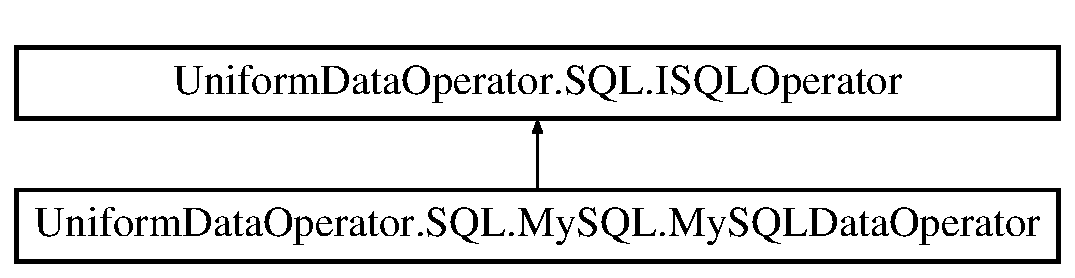
\includegraphics[height=2.000000cm]{de/d4a/interface_uniform_data_operator_1_1_s_q_l_1_1_i_s_q_l_operator}
\end{center}
\end{figure}
\subsection*{Public Member Functions}
\begin{DoxyCompactItemize}
\item 
void \mbox{\hyperlink{interface_uniform_data_operator_1_1_s_q_l_1_1_i_s_q_l_operator_a653f3722befbd300e9ae8ae6f363790f}{Initialize}} ()
\begin{DoxyCompactList}\small\item\em Initialize operator. \end{DoxyCompactList}\item 
bool \mbox{\hyperlink{interface_uniform_data_operator_1_1_s_q_l_1_1_i_s_q_l_operator_aca1b52435a858e57db8d762026ceef2e}{Open\+Connection}} ()
\begin{DoxyCompactList}\small\item\em Opening connection to \mbox{\hyperlink{namespace_uniform_data_operator_1_1_s_q_l}{S\+QL}} server. \end{DoxyCompactList}\item 
bool \mbox{\hyperlink{interface_uniform_data_operator_1_1_s_q_l_1_1_i_s_q_l_operator_a4d13aeb36ebbe0f08eedf48777b048a3}{Close\+Connection}} ()
\begin{DoxyCompactList}\small\item\em Closing connection to \mbox{\hyperlink{namespace_uniform_data_operator_1_1_s_q_l}{S\+QL}} server. \end{DoxyCompactList}\item 
void \mbox{\hyperlink{interface_uniform_data_operator_1_1_s_q_l_1_1_i_s_q_l_operator_a15108adeb878698e82104e374ac37ef2}{Execute\+Non\+Query}} (string query)
\begin{DoxyCompactList}\small\item\em Sending \mbox{\hyperlink{namespace_uniform_data_operator_1_1_s_q_l}{S\+QL}} query to server. \end{DoxyCompactList}\item 
object \mbox{\hyperlink{interface_uniform_data_operator_1_1_s_q_l_1_1_i_s_q_l_operator_a8a39200efe4781edee40151982940f75}{Execute\+Scalar}} (string query)
\begin{DoxyCompactList}\small\item\em Serching for first entry suitable to query and return as result. \end{DoxyCompactList}\item 
Db\+Data\+Reader \mbox{\hyperlink{interface_uniform_data_operator_1_1_s_q_l_1_1_i_s_q_l_operator_a1f6dfa5dd14f7d52559b4e8f1ffda52e}{Execute\+Reader}} (string query)
\begin{DoxyCompactList}\small\item\em Execute complex data reader. \end{DoxyCompactList}\item 
int \mbox{\hyperlink{interface_uniform_data_operator_1_1_s_q_l_1_1_i_s_q_l_operator_a92feb21e03810b152f16f06d02d2034a}{Count}} (string query)
\begin{DoxyCompactList}\small\item\em Try to return count by query. \end{DoxyCompactList}\item 
void \mbox{\hyperlink{interface_uniform_data_operator_1_1_s_q_l_1_1_i_s_q_l_operator_acc29fb7a4b5c3d2dc91d5f9f32b91ca5}{Backup}} (string directory)
\begin{DoxyCompactList}\small\item\em Backuping data base to sql file in directory. Name would be generated by timestamp. \end{DoxyCompactList}\item 
void \mbox{\hyperlink{interface_uniform_data_operator_1_1_s_q_l_1_1_i_s_q_l_operator_ae55ed846c8954ddf7baa6d6dd2e8cb68}{Restore}} (string file\+Path)
\begin{DoxyCompactList}\small\item\em Restoring \mbox{\hyperlink{namespace_uniform_data_operator_1_1_s_q_l}{S\+QL}} db from file. \end{DoxyCompactList}\end{DoxyCompactItemize}
\subsection*{Properties}
\begin{DoxyCompactItemize}
\item 
string \mbox{\hyperlink{interface_uniform_data_operator_1_1_s_q_l_1_1_i_s_q_l_operator_af3e81967d2c0d3457e96d3c41f4c6712}{Server}}\hspace{0.3cm}{\ttfamily  \mbox{[}get, set\mbox{]}}
\begin{DoxyCompactList}\small\item\em Server\textquotesingle{}s ip. \end{DoxyCompactList}\item 
string \mbox{\hyperlink{interface_uniform_data_operator_1_1_s_q_l_1_1_i_s_q_l_operator_a03fee3fec4e4915a540af2b9ac6ecb30}{Database}}\hspace{0.3cm}{\ttfamily  \mbox{[}get, set\mbox{]}}
\begin{DoxyCompactList}\small\item\em Database\textquotesingle{}s name. \end{DoxyCompactList}\item 
string \mbox{\hyperlink{interface_uniform_data_operator_1_1_s_q_l_1_1_i_s_q_l_operator_a47f3c169274d8efefa64a777e0b06b51}{User\+Id}}\hspace{0.3cm}{\ttfamily  \mbox{[}get, set\mbox{]}}
\begin{DoxyCompactList}\small\item\em User for connection. \end{DoxyCompactList}\item 
string \mbox{\hyperlink{interface_uniform_data_operator_1_1_s_q_l_1_1_i_s_q_l_operator_ad4696c7f2d90f7ba0eed37013c812b0a}{Password}}\hspace{0.3cm}{\ttfamily  \mbox{[}get, set\mbox{]}}
\begin{DoxyCompactList}\small\item\em User\textquotesingle{}s password. \end{DoxyCompactList}\end{DoxyCompactItemize}


\subsection{Detailed Description}
Implement that interface to provide possiblity to controll your data base by using \mbox{\hyperlink{namespace_uniform_data_operator_1_1_s_q_l}{S\+QL}} queries. 



\subsection{Member Function Documentation}
\mbox{\Hypertarget{interface_uniform_data_operator_1_1_s_q_l_1_1_i_s_q_l_operator_acc29fb7a4b5c3d2dc91d5f9f32b91ca5}\label{interface_uniform_data_operator_1_1_s_q_l_1_1_i_s_q_l_operator_acc29fb7a4b5c3d2dc91d5f9f32b91ca5}} 
\index{Uniform\+Data\+Operator\+::\+S\+Q\+L\+::\+I\+S\+Q\+L\+Operator@{Uniform\+Data\+Operator\+::\+S\+Q\+L\+::\+I\+S\+Q\+L\+Operator}!Backup@{Backup}}
\index{Backup@{Backup}!Uniform\+Data\+Operator\+::\+S\+Q\+L\+::\+I\+S\+Q\+L\+Operator@{Uniform\+Data\+Operator\+::\+S\+Q\+L\+::\+I\+S\+Q\+L\+Operator}}
\subsubsection{\texorpdfstring{Backup()}{Backup()}}
{\footnotesize\ttfamily void Uniform\+Data\+Operator.\+S\+Q\+L.\+I\+S\+Q\+L\+Operator.\+Backup (\begin{DoxyParamCaption}\item[{string}]{directory }\end{DoxyParamCaption})}



Backuping data base to sql file in directory. Name would be generated by timestamp. 


\begin{DoxyParams}{Parameters}
{\em directory} & Directory that would store the backup file.\\
\hline
\end{DoxyParams}


Implemented in \mbox{\hyperlink{class_uniform_data_operator_1_1_s_q_l_1_1_my_s_q_l_1_1_my_s_q_l_data_operator_a3684b6d5abbcde94880ef433a8ffb28f}{Uniform\+Data\+Operator.\+S\+Q\+L.\+My\+S\+Q\+L.\+My\+S\+Q\+L\+Data\+Operator}}.

\mbox{\Hypertarget{interface_uniform_data_operator_1_1_s_q_l_1_1_i_s_q_l_operator_a4d13aeb36ebbe0f08eedf48777b048a3}\label{interface_uniform_data_operator_1_1_s_q_l_1_1_i_s_q_l_operator_a4d13aeb36ebbe0f08eedf48777b048a3}} 
\index{Uniform\+Data\+Operator\+::\+S\+Q\+L\+::\+I\+S\+Q\+L\+Operator@{Uniform\+Data\+Operator\+::\+S\+Q\+L\+::\+I\+S\+Q\+L\+Operator}!Close\+Connection@{Close\+Connection}}
\index{Close\+Connection@{Close\+Connection}!Uniform\+Data\+Operator\+::\+S\+Q\+L\+::\+I\+S\+Q\+L\+Operator@{Uniform\+Data\+Operator\+::\+S\+Q\+L\+::\+I\+S\+Q\+L\+Operator}}
\subsubsection{\texorpdfstring{Close\+Connection()}{CloseConnection()}}
{\footnotesize\ttfamily bool Uniform\+Data\+Operator.\+S\+Q\+L.\+I\+S\+Q\+L\+Operator.\+Close\+Connection (\begin{DoxyParamCaption}{ }\end{DoxyParamCaption})}



Closing connection to \mbox{\hyperlink{namespace_uniform_data_operator_1_1_s_q_l}{S\+QL}} server. 

\begin{DoxyReturn}{Returns}
Result of connection closing.
\end{DoxyReturn}


Implemented in \mbox{\hyperlink{class_uniform_data_operator_1_1_s_q_l_1_1_my_s_q_l_1_1_my_s_q_l_data_operator_a91ede325ae734daa6a6fff90cab920bc}{Uniform\+Data\+Operator.\+S\+Q\+L.\+My\+S\+Q\+L.\+My\+S\+Q\+L\+Data\+Operator}}.

\mbox{\Hypertarget{interface_uniform_data_operator_1_1_s_q_l_1_1_i_s_q_l_operator_a92feb21e03810b152f16f06d02d2034a}\label{interface_uniform_data_operator_1_1_s_q_l_1_1_i_s_q_l_operator_a92feb21e03810b152f16f06d02d2034a}} 
\index{Uniform\+Data\+Operator\+::\+S\+Q\+L\+::\+I\+S\+Q\+L\+Operator@{Uniform\+Data\+Operator\+::\+S\+Q\+L\+::\+I\+S\+Q\+L\+Operator}!Count@{Count}}
\index{Count@{Count}!Uniform\+Data\+Operator\+::\+S\+Q\+L\+::\+I\+S\+Q\+L\+Operator@{Uniform\+Data\+Operator\+::\+S\+Q\+L\+::\+I\+S\+Q\+L\+Operator}}
\subsubsection{\texorpdfstring{Count()}{Count()}}
{\footnotesize\ttfamily int Uniform\+Data\+Operator.\+S\+Q\+L.\+I\+S\+Q\+L\+Operator.\+Count (\begin{DoxyParamCaption}\item[{string}]{query }\end{DoxyParamCaption})}



Try to return count by query. 


\begin{DoxyParams}{Parameters}
{\em query} & \mbox{\hyperlink{namespace_uniform_data_operator_1_1_s_q_l}{S\+QL}} query that would send to server.\\
\hline
\end{DoxyParams}
\begin{DoxyReturn}{Returns}
Count. -\/1 if not found.
\end{DoxyReturn}


Implemented in \mbox{\hyperlink{class_uniform_data_operator_1_1_s_q_l_1_1_my_s_q_l_1_1_my_s_q_l_data_operator_a05cba564076cc8506ab0272b29f96098}{Uniform\+Data\+Operator.\+S\+Q\+L.\+My\+S\+Q\+L.\+My\+S\+Q\+L\+Data\+Operator}}.

\mbox{\Hypertarget{interface_uniform_data_operator_1_1_s_q_l_1_1_i_s_q_l_operator_a15108adeb878698e82104e374ac37ef2}\label{interface_uniform_data_operator_1_1_s_q_l_1_1_i_s_q_l_operator_a15108adeb878698e82104e374ac37ef2}} 
\index{Uniform\+Data\+Operator\+::\+S\+Q\+L\+::\+I\+S\+Q\+L\+Operator@{Uniform\+Data\+Operator\+::\+S\+Q\+L\+::\+I\+S\+Q\+L\+Operator}!Execute\+Non\+Query@{Execute\+Non\+Query}}
\index{Execute\+Non\+Query@{Execute\+Non\+Query}!Uniform\+Data\+Operator\+::\+S\+Q\+L\+::\+I\+S\+Q\+L\+Operator@{Uniform\+Data\+Operator\+::\+S\+Q\+L\+::\+I\+S\+Q\+L\+Operator}}
\subsubsection{\texorpdfstring{Execute\+Non\+Query()}{ExecuteNonQuery()}}
{\footnotesize\ttfamily void Uniform\+Data\+Operator.\+S\+Q\+L.\+I\+S\+Q\+L\+Operator.\+Execute\+Non\+Query (\begin{DoxyParamCaption}\item[{string}]{query }\end{DoxyParamCaption})}



Sending \mbox{\hyperlink{namespace_uniform_data_operator_1_1_s_q_l}{S\+QL}} query to server. 


\begin{DoxyParams}{Parameters}
{\em query} & \\
\hline
\end{DoxyParams}


Implemented in \mbox{\hyperlink{class_uniform_data_operator_1_1_s_q_l_1_1_my_s_q_l_1_1_my_s_q_l_data_operator_a9e565918b8328323520c6e059d8e3d1f}{Uniform\+Data\+Operator.\+S\+Q\+L.\+My\+S\+Q\+L.\+My\+S\+Q\+L\+Data\+Operator}}.

\mbox{\Hypertarget{interface_uniform_data_operator_1_1_s_q_l_1_1_i_s_q_l_operator_a1f6dfa5dd14f7d52559b4e8f1ffda52e}\label{interface_uniform_data_operator_1_1_s_q_l_1_1_i_s_q_l_operator_a1f6dfa5dd14f7d52559b4e8f1ffda52e}} 
\index{Uniform\+Data\+Operator\+::\+S\+Q\+L\+::\+I\+S\+Q\+L\+Operator@{Uniform\+Data\+Operator\+::\+S\+Q\+L\+::\+I\+S\+Q\+L\+Operator}!Execute\+Reader@{Execute\+Reader}}
\index{Execute\+Reader@{Execute\+Reader}!Uniform\+Data\+Operator\+::\+S\+Q\+L\+::\+I\+S\+Q\+L\+Operator@{Uniform\+Data\+Operator\+::\+S\+Q\+L\+::\+I\+S\+Q\+L\+Operator}}
\subsubsection{\texorpdfstring{Execute\+Reader()}{ExecuteReader()}}
{\footnotesize\ttfamily Db\+Data\+Reader Uniform\+Data\+Operator.\+S\+Q\+L.\+I\+S\+Q\+L\+Operator.\+Execute\+Reader (\begin{DoxyParamCaption}\item[{string}]{query }\end{DoxyParamCaption})}



Execute complex data reader. 


\begin{DoxyParams}{Parameters}
{\em query} & \mbox{\hyperlink{namespace_uniform_data_operator_1_1_s_q_l}{S\+QL}} query that would be shared to server.\\
\hline
\end{DoxyParams}
\begin{DoxyReturn}{Returns}
Data reader with recived data.
\end{DoxyReturn}


Implemented in \mbox{\hyperlink{class_uniform_data_operator_1_1_s_q_l_1_1_my_s_q_l_1_1_my_s_q_l_data_operator_aef1f1d171818fffe2f0c0642de27596d}{Uniform\+Data\+Operator.\+S\+Q\+L.\+My\+S\+Q\+L.\+My\+S\+Q\+L\+Data\+Operator}}.

\mbox{\Hypertarget{interface_uniform_data_operator_1_1_s_q_l_1_1_i_s_q_l_operator_a8a39200efe4781edee40151982940f75}\label{interface_uniform_data_operator_1_1_s_q_l_1_1_i_s_q_l_operator_a8a39200efe4781edee40151982940f75}} 
\index{Uniform\+Data\+Operator\+::\+S\+Q\+L\+::\+I\+S\+Q\+L\+Operator@{Uniform\+Data\+Operator\+::\+S\+Q\+L\+::\+I\+S\+Q\+L\+Operator}!Execute\+Scalar@{Execute\+Scalar}}
\index{Execute\+Scalar@{Execute\+Scalar}!Uniform\+Data\+Operator\+::\+S\+Q\+L\+::\+I\+S\+Q\+L\+Operator@{Uniform\+Data\+Operator\+::\+S\+Q\+L\+::\+I\+S\+Q\+L\+Operator}}
\subsubsection{\texorpdfstring{Execute\+Scalar()}{ExecuteScalar()}}
{\footnotesize\ttfamily object Uniform\+Data\+Operator.\+S\+Q\+L.\+I\+S\+Q\+L\+Operator.\+Execute\+Scalar (\begin{DoxyParamCaption}\item[{string}]{query }\end{DoxyParamCaption})}



Serching for first entry suitable to query and return as result. 


\begin{DoxyParams}{Parameters}
{\em query} & \\
\hline
\end{DoxyParams}
\begin{DoxyReturn}{Returns}
Recived data.
\end{DoxyReturn}


Implemented in \mbox{\hyperlink{class_uniform_data_operator_1_1_s_q_l_1_1_my_s_q_l_1_1_my_s_q_l_data_operator_a0dbc2a3ee5fb7768868138bbd2d9967e}{Uniform\+Data\+Operator.\+S\+Q\+L.\+My\+S\+Q\+L.\+My\+S\+Q\+L\+Data\+Operator}}.

\mbox{\Hypertarget{interface_uniform_data_operator_1_1_s_q_l_1_1_i_s_q_l_operator_a653f3722befbd300e9ae8ae6f363790f}\label{interface_uniform_data_operator_1_1_s_q_l_1_1_i_s_q_l_operator_a653f3722befbd300e9ae8ae6f363790f}} 
\index{Uniform\+Data\+Operator\+::\+S\+Q\+L\+::\+I\+S\+Q\+L\+Operator@{Uniform\+Data\+Operator\+::\+S\+Q\+L\+::\+I\+S\+Q\+L\+Operator}!Initialize@{Initialize}}
\index{Initialize@{Initialize}!Uniform\+Data\+Operator\+::\+S\+Q\+L\+::\+I\+S\+Q\+L\+Operator@{Uniform\+Data\+Operator\+::\+S\+Q\+L\+::\+I\+S\+Q\+L\+Operator}}
\subsubsection{\texorpdfstring{Initialize()}{Initialize()}}
{\footnotesize\ttfamily void Uniform\+Data\+Operator.\+S\+Q\+L.\+I\+S\+Q\+L\+Operator.\+Initialize (\begin{DoxyParamCaption}{ }\end{DoxyParamCaption})}



Initialize operator. 



Implemented in \mbox{\hyperlink{class_uniform_data_operator_1_1_s_q_l_1_1_my_s_q_l_1_1_my_s_q_l_data_operator_a40f968c5e4fd76b611eba5f59faa16c2}{Uniform\+Data\+Operator.\+S\+Q\+L.\+My\+S\+Q\+L.\+My\+S\+Q\+L\+Data\+Operator}}.

\mbox{\Hypertarget{interface_uniform_data_operator_1_1_s_q_l_1_1_i_s_q_l_operator_aca1b52435a858e57db8d762026ceef2e}\label{interface_uniform_data_operator_1_1_s_q_l_1_1_i_s_q_l_operator_aca1b52435a858e57db8d762026ceef2e}} 
\index{Uniform\+Data\+Operator\+::\+S\+Q\+L\+::\+I\+S\+Q\+L\+Operator@{Uniform\+Data\+Operator\+::\+S\+Q\+L\+::\+I\+S\+Q\+L\+Operator}!Open\+Connection@{Open\+Connection}}
\index{Open\+Connection@{Open\+Connection}!Uniform\+Data\+Operator\+::\+S\+Q\+L\+::\+I\+S\+Q\+L\+Operator@{Uniform\+Data\+Operator\+::\+S\+Q\+L\+::\+I\+S\+Q\+L\+Operator}}
\subsubsection{\texorpdfstring{Open\+Connection()}{OpenConnection()}}
{\footnotesize\ttfamily bool Uniform\+Data\+Operator.\+S\+Q\+L.\+I\+S\+Q\+L\+Operator.\+Open\+Connection (\begin{DoxyParamCaption}{ }\end{DoxyParamCaption})}



Opening connection to \mbox{\hyperlink{namespace_uniform_data_operator_1_1_s_q_l}{S\+QL}} server. 

\begin{DoxyReturn}{Returns}
Result of connection.
\end{DoxyReturn}


Implemented in \mbox{\hyperlink{class_uniform_data_operator_1_1_s_q_l_1_1_my_s_q_l_1_1_my_s_q_l_data_operator_acb5a33a4c04bb78290d2ee44ba8479f7}{Uniform\+Data\+Operator.\+S\+Q\+L.\+My\+S\+Q\+L.\+My\+S\+Q\+L\+Data\+Operator}}.

\mbox{\Hypertarget{interface_uniform_data_operator_1_1_s_q_l_1_1_i_s_q_l_operator_ae55ed846c8954ddf7baa6d6dd2e8cb68}\label{interface_uniform_data_operator_1_1_s_q_l_1_1_i_s_q_l_operator_ae55ed846c8954ddf7baa6d6dd2e8cb68}} 
\index{Uniform\+Data\+Operator\+::\+S\+Q\+L\+::\+I\+S\+Q\+L\+Operator@{Uniform\+Data\+Operator\+::\+S\+Q\+L\+::\+I\+S\+Q\+L\+Operator}!Restore@{Restore}}
\index{Restore@{Restore}!Uniform\+Data\+Operator\+::\+S\+Q\+L\+::\+I\+S\+Q\+L\+Operator@{Uniform\+Data\+Operator\+::\+S\+Q\+L\+::\+I\+S\+Q\+L\+Operator}}
\subsubsection{\texorpdfstring{Restore()}{Restore()}}
{\footnotesize\ttfamily void Uniform\+Data\+Operator.\+S\+Q\+L.\+I\+S\+Q\+L\+Operator.\+Restore (\begin{DoxyParamCaption}\item[{string}]{file\+Path }\end{DoxyParamCaption})}



Restoring \mbox{\hyperlink{namespace_uniform_data_operator_1_1_s_q_l}{S\+QL}} db from file. 


\begin{DoxyParams}{Parameters}
{\em file\+Path} & Full path to file\\
\hline
\end{DoxyParams}


Implemented in \mbox{\hyperlink{class_uniform_data_operator_1_1_s_q_l_1_1_my_s_q_l_1_1_my_s_q_l_data_operator_a469885c20c44b1b83d7edc46cda6d539}{Uniform\+Data\+Operator.\+S\+Q\+L.\+My\+S\+Q\+L.\+My\+S\+Q\+L\+Data\+Operator}}.



\subsection{Property Documentation}
\mbox{\Hypertarget{interface_uniform_data_operator_1_1_s_q_l_1_1_i_s_q_l_operator_a03fee3fec4e4915a540af2b9ac6ecb30}\label{interface_uniform_data_operator_1_1_s_q_l_1_1_i_s_q_l_operator_a03fee3fec4e4915a540af2b9ac6ecb30}} 
\index{Uniform\+Data\+Operator\+::\+S\+Q\+L\+::\+I\+S\+Q\+L\+Operator@{Uniform\+Data\+Operator\+::\+S\+Q\+L\+::\+I\+S\+Q\+L\+Operator}!Database@{Database}}
\index{Database@{Database}!Uniform\+Data\+Operator\+::\+S\+Q\+L\+::\+I\+S\+Q\+L\+Operator@{Uniform\+Data\+Operator\+::\+S\+Q\+L\+::\+I\+S\+Q\+L\+Operator}}
\subsubsection{\texorpdfstring{Database}{Database}}
{\footnotesize\ttfamily string Uniform\+Data\+Operator.\+S\+Q\+L.\+I\+S\+Q\+L\+Operator.\+Database\hspace{0.3cm}{\ttfamily [get]}, {\ttfamily [set]}}



Database\textquotesingle{}s name. 

\mbox{\Hypertarget{interface_uniform_data_operator_1_1_s_q_l_1_1_i_s_q_l_operator_ad4696c7f2d90f7ba0eed37013c812b0a}\label{interface_uniform_data_operator_1_1_s_q_l_1_1_i_s_q_l_operator_ad4696c7f2d90f7ba0eed37013c812b0a}} 
\index{Uniform\+Data\+Operator\+::\+S\+Q\+L\+::\+I\+S\+Q\+L\+Operator@{Uniform\+Data\+Operator\+::\+S\+Q\+L\+::\+I\+S\+Q\+L\+Operator}!Password@{Password}}
\index{Password@{Password}!Uniform\+Data\+Operator\+::\+S\+Q\+L\+::\+I\+S\+Q\+L\+Operator@{Uniform\+Data\+Operator\+::\+S\+Q\+L\+::\+I\+S\+Q\+L\+Operator}}
\subsubsection{\texorpdfstring{Password}{Password}}
{\footnotesize\ttfamily string Uniform\+Data\+Operator.\+S\+Q\+L.\+I\+S\+Q\+L\+Operator.\+Password\hspace{0.3cm}{\ttfamily [get]}, {\ttfamily [set]}}



User\textquotesingle{}s password. 

\mbox{\Hypertarget{interface_uniform_data_operator_1_1_s_q_l_1_1_i_s_q_l_operator_af3e81967d2c0d3457e96d3c41f4c6712}\label{interface_uniform_data_operator_1_1_s_q_l_1_1_i_s_q_l_operator_af3e81967d2c0d3457e96d3c41f4c6712}} 
\index{Uniform\+Data\+Operator\+::\+S\+Q\+L\+::\+I\+S\+Q\+L\+Operator@{Uniform\+Data\+Operator\+::\+S\+Q\+L\+::\+I\+S\+Q\+L\+Operator}!Server@{Server}}
\index{Server@{Server}!Uniform\+Data\+Operator\+::\+S\+Q\+L\+::\+I\+S\+Q\+L\+Operator@{Uniform\+Data\+Operator\+::\+S\+Q\+L\+::\+I\+S\+Q\+L\+Operator}}
\subsubsection{\texorpdfstring{Server}{Server}}
{\footnotesize\ttfamily string Uniform\+Data\+Operator.\+S\+Q\+L.\+I\+S\+Q\+L\+Operator.\+Server\hspace{0.3cm}{\ttfamily [get]}, {\ttfamily [set]}}



Server\textquotesingle{}s ip. 

\mbox{\Hypertarget{interface_uniform_data_operator_1_1_s_q_l_1_1_i_s_q_l_operator_a47f3c169274d8efefa64a777e0b06b51}\label{interface_uniform_data_operator_1_1_s_q_l_1_1_i_s_q_l_operator_a47f3c169274d8efefa64a777e0b06b51}} 
\index{Uniform\+Data\+Operator\+::\+S\+Q\+L\+::\+I\+S\+Q\+L\+Operator@{Uniform\+Data\+Operator\+::\+S\+Q\+L\+::\+I\+S\+Q\+L\+Operator}!User\+Id@{User\+Id}}
\index{User\+Id@{User\+Id}!Uniform\+Data\+Operator\+::\+S\+Q\+L\+::\+I\+S\+Q\+L\+Operator@{Uniform\+Data\+Operator\+::\+S\+Q\+L\+::\+I\+S\+Q\+L\+Operator}}
\subsubsection{\texorpdfstring{User\+Id}{UserId}}
{\footnotesize\ttfamily string Uniform\+Data\+Operator.\+S\+Q\+L.\+I\+S\+Q\+L\+Operator.\+User\+Id\hspace{0.3cm}{\ttfamily [get]}, {\ttfamily [set]}}



User for connection. 



The documentation for this interface was generated from the following file\+:\begin{DoxyCompactItemize}
\item 
D\+:/\+Work/\+Git\+Hub/uniform-\/data-\/operator/\+S\+Q\+L/I\+S\+Q\+L\+Operator.\+cs\end{DoxyCompactItemize}

\hypertarget{interface_uniform_data_operator_1_1_s_q_l_1_1_tables_1_1_i_s_q_l_table}{}\section{Uniform\+Data\+Operator.\+S\+Q\+L.\+Tables.\+I\+S\+Q\+L\+Table Interface Reference}
\label{interface_uniform_data_operator_1_1_s_q_l_1_1_tables_1_1_i_s_q_l_table}\index{Uniform\+Data\+Operator.\+S\+Q\+L.\+Tables.\+I\+S\+Q\+L\+Table@{Uniform\+Data\+Operator.\+S\+Q\+L.\+Tables.\+I\+S\+Q\+L\+Table}}


Interface that allow to get description of target table required for object.  


\subsection*{Properties}
\begin{DoxyCompactItemize}
\item 
string \mbox{\hyperlink{interface_uniform_data_operator_1_1_s_q_l_1_1_tables_1_1_i_s_q_l_table_afe5c80cd1f594bfdd6f0ba3d9ffaf674}{Schema\+Name}}\hspace{0.3cm}{\ttfamily  \mbox{[}get\mbox{]}}
\begin{DoxyCompactList}\small\item\em Name of the target schema. \end{DoxyCompactList}\item 
string \mbox{\hyperlink{interface_uniform_data_operator_1_1_s_q_l_1_1_tables_1_1_i_s_q_l_table_ae29ed8f9fa5796db79a6f30c2006d79a}{Table\+Name}}\hspace{0.3cm}{\ttfamily  \mbox{[}get\mbox{]}}
\begin{DoxyCompactList}\small\item\em Name of the table. \end{DoxyCompactList}\item 
string \mbox{\hyperlink{interface_uniform_data_operator_1_1_s_q_l_1_1_tables_1_1_i_s_q_l_table_a13b1d02d264dc49bf8998a2c84e491d4}{Table\+Engine}}\hspace{0.3cm}{\ttfamily  \mbox{[}get\mbox{]}}
\begin{DoxyCompactList}\small\item\em Engine of this table. Inno\+DB by default. \end{DoxyCompactList}\item 
\mbox{\hyperlink{struct_uniform_data_operator_1_1_s_q_l_1_1_tables_1_1_table_column_meta}{Table\+Column\+Meta}} \mbox{[}$\,$\mbox{]} \mbox{\hyperlink{interface_uniform_data_operator_1_1_s_q_l_1_1_tables_1_1_i_s_q_l_table_a7cd3fd1a60284eb30b48fb7deabec462}{Table\+Fields}}\hspace{0.3cm}{\ttfamily  \mbox{[}get\mbox{]}}
\begin{DoxyCompactList}\small\item\em Array of table fields names. \end{DoxyCompactList}\end{DoxyCompactItemize}


\subsection{Detailed Description}
Interface that allow to get description of target table required for object. 



\subsection{Property Documentation}
\mbox{\Hypertarget{interface_uniform_data_operator_1_1_s_q_l_1_1_tables_1_1_i_s_q_l_table_afe5c80cd1f594bfdd6f0ba3d9ffaf674}\label{interface_uniform_data_operator_1_1_s_q_l_1_1_tables_1_1_i_s_q_l_table_afe5c80cd1f594bfdd6f0ba3d9ffaf674}} 
\index{Uniform\+Data\+Operator\+::\+S\+Q\+L\+::\+Tables\+::\+I\+S\+Q\+L\+Table@{Uniform\+Data\+Operator\+::\+S\+Q\+L\+::\+Tables\+::\+I\+S\+Q\+L\+Table}!Schema\+Name@{Schema\+Name}}
\index{Schema\+Name@{Schema\+Name}!Uniform\+Data\+Operator\+::\+S\+Q\+L\+::\+Tables\+::\+I\+S\+Q\+L\+Table@{Uniform\+Data\+Operator\+::\+S\+Q\+L\+::\+Tables\+::\+I\+S\+Q\+L\+Table}}
\subsubsection{\texorpdfstring{Schema\+Name}{SchemaName}}
{\footnotesize\ttfamily string Uniform\+Data\+Operator.\+S\+Q\+L.\+Tables.\+I\+S\+Q\+L\+Table.\+Schema\+Name\hspace{0.3cm}{\ttfamily [get]}}



Name of the target schema. 

\mbox{\Hypertarget{interface_uniform_data_operator_1_1_s_q_l_1_1_tables_1_1_i_s_q_l_table_a13b1d02d264dc49bf8998a2c84e491d4}\label{interface_uniform_data_operator_1_1_s_q_l_1_1_tables_1_1_i_s_q_l_table_a13b1d02d264dc49bf8998a2c84e491d4}} 
\index{Uniform\+Data\+Operator\+::\+S\+Q\+L\+::\+Tables\+::\+I\+S\+Q\+L\+Table@{Uniform\+Data\+Operator\+::\+S\+Q\+L\+::\+Tables\+::\+I\+S\+Q\+L\+Table}!Table\+Engine@{Table\+Engine}}
\index{Table\+Engine@{Table\+Engine}!Uniform\+Data\+Operator\+::\+S\+Q\+L\+::\+Tables\+::\+I\+S\+Q\+L\+Table@{Uniform\+Data\+Operator\+::\+S\+Q\+L\+::\+Tables\+::\+I\+S\+Q\+L\+Table}}
\subsubsection{\texorpdfstring{Table\+Engine}{TableEngine}}
{\footnotesize\ttfamily string Uniform\+Data\+Operator.\+S\+Q\+L.\+Tables.\+I\+S\+Q\+L\+Table.\+Table\+Engine\hspace{0.3cm}{\ttfamily [get]}}



Engine of this table. Inno\+DB by default. 

\mbox{\Hypertarget{interface_uniform_data_operator_1_1_s_q_l_1_1_tables_1_1_i_s_q_l_table_a7cd3fd1a60284eb30b48fb7deabec462}\label{interface_uniform_data_operator_1_1_s_q_l_1_1_tables_1_1_i_s_q_l_table_a7cd3fd1a60284eb30b48fb7deabec462}} 
\index{Uniform\+Data\+Operator\+::\+S\+Q\+L\+::\+Tables\+::\+I\+S\+Q\+L\+Table@{Uniform\+Data\+Operator\+::\+S\+Q\+L\+::\+Tables\+::\+I\+S\+Q\+L\+Table}!Table\+Fields@{Table\+Fields}}
\index{Table\+Fields@{Table\+Fields}!Uniform\+Data\+Operator\+::\+S\+Q\+L\+::\+Tables\+::\+I\+S\+Q\+L\+Table@{Uniform\+Data\+Operator\+::\+S\+Q\+L\+::\+Tables\+::\+I\+S\+Q\+L\+Table}}
\subsubsection{\texorpdfstring{Table\+Fields}{TableFields}}
{\footnotesize\ttfamily \mbox{\hyperlink{struct_uniform_data_operator_1_1_s_q_l_1_1_tables_1_1_table_column_meta}{Table\+Column\+Meta}} \mbox{[}$\,$\mbox{]} Uniform\+Data\+Operator.\+S\+Q\+L.\+Tables.\+I\+S\+Q\+L\+Table.\+Table\+Fields\hspace{0.3cm}{\ttfamily [get]}}



Array of table fields names. 

\mbox{\Hypertarget{interface_uniform_data_operator_1_1_s_q_l_1_1_tables_1_1_i_s_q_l_table_ae29ed8f9fa5796db79a6f30c2006d79a}\label{interface_uniform_data_operator_1_1_s_q_l_1_1_tables_1_1_i_s_q_l_table_ae29ed8f9fa5796db79a6f30c2006d79a}} 
\index{Uniform\+Data\+Operator\+::\+S\+Q\+L\+::\+Tables\+::\+I\+S\+Q\+L\+Table@{Uniform\+Data\+Operator\+::\+S\+Q\+L\+::\+Tables\+::\+I\+S\+Q\+L\+Table}!Table\+Name@{Table\+Name}}
\index{Table\+Name@{Table\+Name}!Uniform\+Data\+Operator\+::\+S\+Q\+L\+::\+Tables\+::\+I\+S\+Q\+L\+Table@{Uniform\+Data\+Operator\+::\+S\+Q\+L\+::\+Tables\+::\+I\+S\+Q\+L\+Table}}
\subsubsection{\texorpdfstring{Table\+Name}{TableName}}
{\footnotesize\ttfamily string Uniform\+Data\+Operator.\+S\+Q\+L.\+Tables.\+I\+S\+Q\+L\+Table.\+Table\+Name\hspace{0.3cm}{\ttfamily [get]}}



Name of the table. 



The documentation for this interface was generated from the following file\+:\begin{DoxyCompactItemize}
\item 
D\+:/\+Work/\+Git\+Hub/uniform-\/data-\/operator/\+S\+Q\+L/\+Tables/I\+S\+Q\+L\+Table.\+cs\end{DoxyCompactItemize}

\hypertarget{class_uniform_data_operator_1_1_s_q_l_1_1_my_s_q_l_1_1_my_s_q_l_data_operator}{}\section{Uniform\+Data\+Operator.\+S\+Q\+L.\+My\+S\+Q\+L.\+My\+S\+Q\+L\+Data\+Operator Class Reference}
\label{class_uniform_data_operator_1_1_s_q_l_1_1_my_s_q_l_1_1_my_s_q_l_data_operator}\index{Uniform\+Data\+Operator.\+S\+Q\+L.\+My\+S\+Q\+L.\+My\+S\+Q\+L\+Data\+Operator@{Uniform\+Data\+Operator.\+S\+Q\+L.\+My\+S\+Q\+L.\+My\+S\+Q\+L\+Data\+Operator}}


Operator that provides possibility to operate data on \mbox{\hyperlink{namespace_uniform_data_operator_1_1_s_q_l_1_1_my_s_q_l}{My\+S\+QL}} data base server.  


Inheritance diagram for Uniform\+Data\+Operator.\+S\+Q\+L.\+My\+S\+Q\+L.\+My\+S\+Q\+L\+Data\+Operator\+:\begin{figure}[H]
\begin{center}
\leavevmode
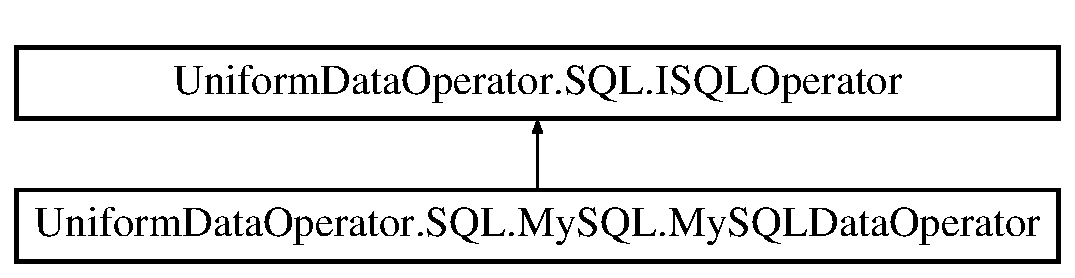
\includegraphics[height=2.000000cm]{d9/d5d/class_uniform_data_operator_1_1_s_q_l_1_1_my_s_q_l_1_1_my_s_q_l_data_operator}
\end{center}
\end{figure}
\subsection*{Public Member Functions}
\begin{DoxyCompactItemize}
\item 
void \mbox{\hyperlink{class_uniform_data_operator_1_1_s_q_l_1_1_my_s_q_l_1_1_my_s_q_l_data_operator_a40f968c5e4fd76b611eba5f59faa16c2}{Initialize}} ()
\begin{DoxyCompactList}\small\item\em Initialize My\+Sql\+Connection. \end{DoxyCompactList}\item 
bool \mbox{\hyperlink{class_uniform_data_operator_1_1_s_q_l_1_1_my_s_q_l_1_1_my_s_q_l_data_operator_acb5a33a4c04bb78290d2ee44ba8479f7}{Open\+Connection}} ()
\begin{DoxyCompactList}\small\item\em Opening connection to \mbox{\hyperlink{namespace_uniform_data_operator_1_1_s_q_l}{S\+QL}} server. \end{DoxyCompactList}\item 
bool \mbox{\hyperlink{class_uniform_data_operator_1_1_s_q_l_1_1_my_s_q_l_1_1_my_s_q_l_data_operator_a91ede325ae734daa6a6fff90cab920bc}{Close\+Connection}} ()
\begin{DoxyCompactList}\small\item\em Closing connection to \mbox{\hyperlink{namespace_uniform_data_operator_1_1_s_q_l}{S\+QL}} server. \end{DoxyCompactList}\item 
void \mbox{\hyperlink{class_uniform_data_operator_1_1_s_q_l_1_1_my_s_q_l_1_1_my_s_q_l_data_operator_a9e565918b8328323520c6e059d8e3d1f}{Execute\+Non\+Query}} (string query)
\begin{DoxyCompactList}\small\item\em Sending \mbox{\hyperlink{namespace_uniform_data_operator_1_1_s_q_l}{S\+QL}} query to server. \end{DoxyCompactList}\item 
object \mbox{\hyperlink{class_uniform_data_operator_1_1_s_q_l_1_1_my_s_q_l_1_1_my_s_q_l_data_operator_a0dbc2a3ee5fb7768868138bbd2d9967e}{Execute\+Scalar}} (string query)
\begin{DoxyCompactList}\small\item\em Serching for first entry suitable to query and return as result. \end{DoxyCompactList}\item 
Db\+Data\+Reader \mbox{\hyperlink{class_uniform_data_operator_1_1_s_q_l_1_1_my_s_q_l_1_1_my_s_q_l_data_operator_aef1f1d171818fffe2f0c0642de27596d}{Execute\+Reader}} (string query)
\begin{DoxyCompactList}\small\item\em Execute complex data reader. \end{DoxyCompactList}\item 
int \mbox{\hyperlink{class_uniform_data_operator_1_1_s_q_l_1_1_my_s_q_l_1_1_my_s_q_l_data_operator_a05cba564076cc8506ab0272b29f96098}{Count}} (string query)
\begin{DoxyCompactList}\small\item\em Try to return count by query. \end{DoxyCompactList}\item 
void \mbox{\hyperlink{class_uniform_data_operator_1_1_s_q_l_1_1_my_s_q_l_1_1_my_s_q_l_data_operator_a3684b6d5abbcde94880ef433a8ffb28f}{Backup}} (string directory)
\begin{DoxyCompactList}\small\item\em Backuping data base to sql file in directory. Name would be generated by timestamp. \end{DoxyCompactList}\item 
void \mbox{\hyperlink{class_uniform_data_operator_1_1_s_q_l_1_1_my_s_q_l_1_1_my_s_q_l_data_operator_a469885c20c44b1b83d7edc46cda6d539}{Restore}} (string file\+Path)
\begin{DoxyCompactList}\small\item\em Restoring \mbox{\hyperlink{namespace_uniform_data_operator_1_1_s_q_l}{S\+QL}} db from file. \end{DoxyCompactList}\end{DoxyCompactItemize}
\subsection*{Properties}
\begin{DoxyCompactItemize}
\item 
static \mbox{\hyperlink{class_uniform_data_operator_1_1_s_q_l_1_1_my_s_q_l_1_1_my_s_q_l_data_operator}{My\+S\+Q\+L\+Data\+Operator}} \mbox{\hyperlink{class_uniform_data_operator_1_1_s_q_l_1_1_my_s_q_l_1_1_my_s_q_l_data_operator_aa9f199b686be335bb2828893f7ad2a90}{Active}}\hspace{0.3cm}{\ttfamily  \mbox{[}get\mbox{]}}
\begin{DoxyCompactList}\small\item\em Active single tone instance of \mbox{\hyperlink{namespace_uniform_data_operator_1_1_s_q_l_1_1_my_s_q_l}{My\+S\+QL}} data provider. \end{DoxyCompactList}\item 
string \mbox{\hyperlink{class_uniform_data_operator_1_1_s_q_l_1_1_my_s_q_l_1_1_my_s_q_l_data_operator_a14653be731b7636d2c1dd7ed31daba48}{Server}}\hspace{0.3cm}{\ttfamily  \mbox{[}get, set\mbox{]}}
\begin{DoxyCompactList}\small\item\em Server\textquotesingle{}s ip. \end{DoxyCompactList}\item 
string \mbox{\hyperlink{class_uniform_data_operator_1_1_s_q_l_1_1_my_s_q_l_1_1_my_s_q_l_data_operator_a070214377e958a70594e877dba859449}{Database}}\hspace{0.3cm}{\ttfamily  \mbox{[}get, set\mbox{]}}
\begin{DoxyCompactList}\small\item\em Database\textquotesingle{}s name. \end{DoxyCompactList}\item 
string \mbox{\hyperlink{class_uniform_data_operator_1_1_s_q_l_1_1_my_s_q_l_1_1_my_s_q_l_data_operator_ace67458f32cee24fd48f0cc409f4b45a}{User\+Id}}\hspace{0.3cm}{\ttfamily  \mbox{[}get, set\mbox{]}}
\begin{DoxyCompactList}\small\item\em User for connection. \end{DoxyCompactList}\item 
string \mbox{\hyperlink{class_uniform_data_operator_1_1_s_q_l_1_1_my_s_q_l_1_1_my_s_q_l_data_operator_a40b331c12f0b184e3bf771a73e4c2bfd}{Password}}\hspace{0.3cm}{\ttfamily  \mbox{[}get, set\mbox{]}}
\begin{DoxyCompactList}\small\item\em User\textquotesingle{}s password. \end{DoxyCompactList}\end{DoxyCompactItemize}
\subsection*{Private Attributes}
\begin{DoxyCompactItemize}
\item 
My\+Sql\+Connection \mbox{\hyperlink{class_uniform_data_operator_1_1_s_q_l_1_1_my_s_q_l_1_1_my_s_q_l_data_operator_acdc80f644c1a4bc7d8cf71705d513aff}{connection}}
\begin{DoxyCompactList}\small\item\em Object that managing connection with DB. \end{DoxyCompactList}\end{DoxyCompactItemize}
\subsection*{Static Private Attributes}
\begin{DoxyCompactItemize}
\item 
\mbox{\Hypertarget{class_uniform_data_operator_1_1_s_q_l_1_1_my_s_q_l_1_1_my_s_q_l_data_operator_a006ae5b7a455a4409ab7e9551ad6d33c}\label{class_uniform_data_operator_1_1_s_q_l_1_1_my_s_q_l_1_1_my_s_q_l_data_operator_a006ae5b7a455a4409ab7e9551ad6d33c}} 
static \mbox{\hyperlink{class_uniform_data_operator_1_1_s_q_l_1_1_my_s_q_l_1_1_my_s_q_l_data_operator}{My\+S\+Q\+L\+Data\+Operator}} {\bfseries \+\_\+\+Active}
\end{DoxyCompactItemize}


\subsection{Detailed Description}
Operator that provides possibility to operate data on \mbox{\hyperlink{namespace_uniform_data_operator_1_1_s_q_l_1_1_my_s_q_l}{My\+S\+QL}} data base server. 



\subsection{Member Function Documentation}
\mbox{\Hypertarget{class_uniform_data_operator_1_1_s_q_l_1_1_my_s_q_l_1_1_my_s_q_l_data_operator_a3684b6d5abbcde94880ef433a8ffb28f}\label{class_uniform_data_operator_1_1_s_q_l_1_1_my_s_q_l_1_1_my_s_q_l_data_operator_a3684b6d5abbcde94880ef433a8ffb28f}} 
\index{Uniform\+Data\+Operator\+::\+S\+Q\+L\+::\+My\+S\+Q\+L\+::\+My\+S\+Q\+L\+Data\+Operator@{Uniform\+Data\+Operator\+::\+S\+Q\+L\+::\+My\+S\+Q\+L\+::\+My\+S\+Q\+L\+Data\+Operator}!Backup@{Backup}}
\index{Backup@{Backup}!Uniform\+Data\+Operator\+::\+S\+Q\+L\+::\+My\+S\+Q\+L\+::\+My\+S\+Q\+L\+Data\+Operator@{Uniform\+Data\+Operator\+::\+S\+Q\+L\+::\+My\+S\+Q\+L\+::\+My\+S\+Q\+L\+Data\+Operator}}
\subsubsection{\texorpdfstring{Backup()}{Backup()}}
{\footnotesize\ttfamily void Uniform\+Data\+Operator.\+S\+Q\+L.\+My\+S\+Q\+L.\+My\+S\+Q\+L\+Data\+Operator.\+Backup (\begin{DoxyParamCaption}\item[{string}]{directory }\end{DoxyParamCaption})}



Backuping data base to sql file in directory. Name would be generated by timestamp. 


\begin{DoxyParams}{Parameters}
{\em directory} & Directory that would store the backup file.\\
\hline
\end{DoxyParams}


Implements \mbox{\hyperlink{interface_uniform_data_operator_1_1_s_q_l_1_1_i_s_q_l_operator_acc29fb7a4b5c3d2dc91d5f9f32b91ca5}{Uniform\+Data\+Operator.\+S\+Q\+L.\+I\+S\+Q\+L\+Operator}}.

\mbox{\Hypertarget{class_uniform_data_operator_1_1_s_q_l_1_1_my_s_q_l_1_1_my_s_q_l_data_operator_a91ede325ae734daa6a6fff90cab920bc}\label{class_uniform_data_operator_1_1_s_q_l_1_1_my_s_q_l_1_1_my_s_q_l_data_operator_a91ede325ae734daa6a6fff90cab920bc}} 
\index{Uniform\+Data\+Operator\+::\+S\+Q\+L\+::\+My\+S\+Q\+L\+::\+My\+S\+Q\+L\+Data\+Operator@{Uniform\+Data\+Operator\+::\+S\+Q\+L\+::\+My\+S\+Q\+L\+::\+My\+S\+Q\+L\+Data\+Operator}!Close\+Connection@{Close\+Connection}}
\index{Close\+Connection@{Close\+Connection}!Uniform\+Data\+Operator\+::\+S\+Q\+L\+::\+My\+S\+Q\+L\+::\+My\+S\+Q\+L\+Data\+Operator@{Uniform\+Data\+Operator\+::\+S\+Q\+L\+::\+My\+S\+Q\+L\+::\+My\+S\+Q\+L\+Data\+Operator}}
\subsubsection{\texorpdfstring{Close\+Connection()}{CloseConnection()}}
{\footnotesize\ttfamily bool Uniform\+Data\+Operator.\+S\+Q\+L.\+My\+S\+Q\+L.\+My\+S\+Q\+L\+Data\+Operator.\+Close\+Connection (\begin{DoxyParamCaption}{ }\end{DoxyParamCaption})}



Closing connection to \mbox{\hyperlink{namespace_uniform_data_operator_1_1_s_q_l}{S\+QL}} server. 

\begin{DoxyReturn}{Returns}
Result of connection closing.
\end{DoxyReturn}


Implements \mbox{\hyperlink{interface_uniform_data_operator_1_1_s_q_l_1_1_i_s_q_l_operator_a4d13aeb36ebbe0f08eedf48777b048a3}{Uniform\+Data\+Operator.\+S\+Q\+L.\+I\+S\+Q\+L\+Operator}}.

\mbox{\Hypertarget{class_uniform_data_operator_1_1_s_q_l_1_1_my_s_q_l_1_1_my_s_q_l_data_operator_a05cba564076cc8506ab0272b29f96098}\label{class_uniform_data_operator_1_1_s_q_l_1_1_my_s_q_l_1_1_my_s_q_l_data_operator_a05cba564076cc8506ab0272b29f96098}} 
\index{Uniform\+Data\+Operator\+::\+S\+Q\+L\+::\+My\+S\+Q\+L\+::\+My\+S\+Q\+L\+Data\+Operator@{Uniform\+Data\+Operator\+::\+S\+Q\+L\+::\+My\+S\+Q\+L\+::\+My\+S\+Q\+L\+Data\+Operator}!Count@{Count}}
\index{Count@{Count}!Uniform\+Data\+Operator\+::\+S\+Q\+L\+::\+My\+S\+Q\+L\+::\+My\+S\+Q\+L\+Data\+Operator@{Uniform\+Data\+Operator\+::\+S\+Q\+L\+::\+My\+S\+Q\+L\+::\+My\+S\+Q\+L\+Data\+Operator}}
\subsubsection{\texorpdfstring{Count()}{Count()}}
{\footnotesize\ttfamily int Uniform\+Data\+Operator.\+S\+Q\+L.\+My\+S\+Q\+L.\+My\+S\+Q\+L\+Data\+Operator.\+Count (\begin{DoxyParamCaption}\item[{string}]{query }\end{DoxyParamCaption})}



Try to return count by query. 


\begin{DoxyParams}{Parameters}
{\em query} & \mbox{\hyperlink{namespace_uniform_data_operator_1_1_s_q_l}{S\+QL}} query that would send to server.\\
\hline
\end{DoxyParams}
\begin{DoxyReturn}{Returns}
Count. -\/1 by default.
\end{DoxyReturn}


Implements \mbox{\hyperlink{interface_uniform_data_operator_1_1_s_q_l_1_1_i_s_q_l_operator_a92feb21e03810b152f16f06d02d2034a}{Uniform\+Data\+Operator.\+S\+Q\+L.\+I\+S\+Q\+L\+Operator}}.

\mbox{\Hypertarget{class_uniform_data_operator_1_1_s_q_l_1_1_my_s_q_l_1_1_my_s_q_l_data_operator_a9e565918b8328323520c6e059d8e3d1f}\label{class_uniform_data_operator_1_1_s_q_l_1_1_my_s_q_l_1_1_my_s_q_l_data_operator_a9e565918b8328323520c6e059d8e3d1f}} 
\index{Uniform\+Data\+Operator\+::\+S\+Q\+L\+::\+My\+S\+Q\+L\+::\+My\+S\+Q\+L\+Data\+Operator@{Uniform\+Data\+Operator\+::\+S\+Q\+L\+::\+My\+S\+Q\+L\+::\+My\+S\+Q\+L\+Data\+Operator}!Execute\+Non\+Query@{Execute\+Non\+Query}}
\index{Execute\+Non\+Query@{Execute\+Non\+Query}!Uniform\+Data\+Operator\+::\+S\+Q\+L\+::\+My\+S\+Q\+L\+::\+My\+S\+Q\+L\+Data\+Operator@{Uniform\+Data\+Operator\+::\+S\+Q\+L\+::\+My\+S\+Q\+L\+::\+My\+S\+Q\+L\+Data\+Operator}}
\subsubsection{\texorpdfstring{Execute\+Non\+Query()}{ExecuteNonQuery()}}
{\footnotesize\ttfamily void Uniform\+Data\+Operator.\+S\+Q\+L.\+My\+S\+Q\+L.\+My\+S\+Q\+L\+Data\+Operator.\+Execute\+Non\+Query (\begin{DoxyParamCaption}\item[{string}]{query }\end{DoxyParamCaption})}



Sending \mbox{\hyperlink{namespace_uniform_data_operator_1_1_s_q_l}{S\+QL}} query to server. 


\begin{DoxyParams}{Parameters}
{\em query} & \\
\hline
\end{DoxyParams}


Implements \mbox{\hyperlink{interface_uniform_data_operator_1_1_s_q_l_1_1_i_s_q_l_operator_a15108adeb878698e82104e374ac37ef2}{Uniform\+Data\+Operator.\+S\+Q\+L.\+I\+S\+Q\+L\+Operator}}.

\mbox{\Hypertarget{class_uniform_data_operator_1_1_s_q_l_1_1_my_s_q_l_1_1_my_s_q_l_data_operator_aef1f1d171818fffe2f0c0642de27596d}\label{class_uniform_data_operator_1_1_s_q_l_1_1_my_s_q_l_1_1_my_s_q_l_data_operator_aef1f1d171818fffe2f0c0642de27596d}} 
\index{Uniform\+Data\+Operator\+::\+S\+Q\+L\+::\+My\+S\+Q\+L\+::\+My\+S\+Q\+L\+Data\+Operator@{Uniform\+Data\+Operator\+::\+S\+Q\+L\+::\+My\+S\+Q\+L\+::\+My\+S\+Q\+L\+Data\+Operator}!Execute\+Reader@{Execute\+Reader}}
\index{Execute\+Reader@{Execute\+Reader}!Uniform\+Data\+Operator\+::\+S\+Q\+L\+::\+My\+S\+Q\+L\+::\+My\+S\+Q\+L\+Data\+Operator@{Uniform\+Data\+Operator\+::\+S\+Q\+L\+::\+My\+S\+Q\+L\+::\+My\+S\+Q\+L\+Data\+Operator}}
\subsubsection{\texorpdfstring{Execute\+Reader()}{ExecuteReader()}}
{\footnotesize\ttfamily Db\+Data\+Reader Uniform\+Data\+Operator.\+S\+Q\+L.\+My\+S\+Q\+L.\+My\+S\+Q\+L\+Data\+Operator.\+Execute\+Reader (\begin{DoxyParamCaption}\item[{string}]{query }\end{DoxyParamCaption})}



Execute complex data reader. 


\begin{DoxyParams}{Parameters}
{\em query} & \mbox{\hyperlink{namespace_uniform_data_operator_1_1_s_q_l}{S\+QL}} query that would be shared to server.\\
\hline
\end{DoxyParams}
\begin{DoxyReturn}{Returns}
Data reader with recived data.
\end{DoxyReturn}


Implements \mbox{\hyperlink{interface_uniform_data_operator_1_1_s_q_l_1_1_i_s_q_l_operator_a1f6dfa5dd14f7d52559b4e8f1ffda52e}{Uniform\+Data\+Operator.\+S\+Q\+L.\+I\+S\+Q\+L\+Operator}}.

\mbox{\Hypertarget{class_uniform_data_operator_1_1_s_q_l_1_1_my_s_q_l_1_1_my_s_q_l_data_operator_a0dbc2a3ee5fb7768868138bbd2d9967e}\label{class_uniform_data_operator_1_1_s_q_l_1_1_my_s_q_l_1_1_my_s_q_l_data_operator_a0dbc2a3ee5fb7768868138bbd2d9967e}} 
\index{Uniform\+Data\+Operator\+::\+S\+Q\+L\+::\+My\+S\+Q\+L\+::\+My\+S\+Q\+L\+Data\+Operator@{Uniform\+Data\+Operator\+::\+S\+Q\+L\+::\+My\+S\+Q\+L\+::\+My\+S\+Q\+L\+Data\+Operator}!Execute\+Scalar@{Execute\+Scalar}}
\index{Execute\+Scalar@{Execute\+Scalar}!Uniform\+Data\+Operator\+::\+S\+Q\+L\+::\+My\+S\+Q\+L\+::\+My\+S\+Q\+L\+Data\+Operator@{Uniform\+Data\+Operator\+::\+S\+Q\+L\+::\+My\+S\+Q\+L\+::\+My\+S\+Q\+L\+Data\+Operator}}
\subsubsection{\texorpdfstring{Execute\+Scalar()}{ExecuteScalar()}}
{\footnotesize\ttfamily object Uniform\+Data\+Operator.\+S\+Q\+L.\+My\+S\+Q\+L.\+My\+S\+Q\+L\+Data\+Operator.\+Execute\+Scalar (\begin{DoxyParamCaption}\item[{string}]{query }\end{DoxyParamCaption})}



Serching for first entry suitable to query and return as result. 


\begin{DoxyParams}{Parameters}
{\em query} & \\
\hline
\end{DoxyParams}
\begin{DoxyReturn}{Returns}
Recived data.
\end{DoxyReturn}


Implements \mbox{\hyperlink{interface_uniform_data_operator_1_1_s_q_l_1_1_i_s_q_l_operator_a8a39200efe4781edee40151982940f75}{Uniform\+Data\+Operator.\+S\+Q\+L.\+I\+S\+Q\+L\+Operator}}.

\mbox{\Hypertarget{class_uniform_data_operator_1_1_s_q_l_1_1_my_s_q_l_1_1_my_s_q_l_data_operator_a40f968c5e4fd76b611eba5f59faa16c2}\label{class_uniform_data_operator_1_1_s_q_l_1_1_my_s_q_l_1_1_my_s_q_l_data_operator_a40f968c5e4fd76b611eba5f59faa16c2}} 
\index{Uniform\+Data\+Operator\+::\+S\+Q\+L\+::\+My\+S\+Q\+L\+::\+My\+S\+Q\+L\+Data\+Operator@{Uniform\+Data\+Operator\+::\+S\+Q\+L\+::\+My\+S\+Q\+L\+::\+My\+S\+Q\+L\+Data\+Operator}!Initialize@{Initialize}}
\index{Initialize@{Initialize}!Uniform\+Data\+Operator\+::\+S\+Q\+L\+::\+My\+S\+Q\+L\+::\+My\+S\+Q\+L\+Data\+Operator@{Uniform\+Data\+Operator\+::\+S\+Q\+L\+::\+My\+S\+Q\+L\+::\+My\+S\+Q\+L\+Data\+Operator}}
\subsubsection{\texorpdfstring{Initialize()}{Initialize()}}
{\footnotesize\ttfamily void Uniform\+Data\+Operator.\+S\+Q\+L.\+My\+S\+Q\+L.\+My\+S\+Q\+L\+Data\+Operator.\+Initialize (\begin{DoxyParamCaption}{ }\end{DoxyParamCaption})}



Initialize My\+Sql\+Connection. 



Implements \mbox{\hyperlink{interface_uniform_data_operator_1_1_s_q_l_1_1_i_s_q_l_operator_a653f3722befbd300e9ae8ae6f363790f}{Uniform\+Data\+Operator.\+S\+Q\+L.\+I\+S\+Q\+L\+Operator}}.

\mbox{\Hypertarget{class_uniform_data_operator_1_1_s_q_l_1_1_my_s_q_l_1_1_my_s_q_l_data_operator_acb5a33a4c04bb78290d2ee44ba8479f7}\label{class_uniform_data_operator_1_1_s_q_l_1_1_my_s_q_l_1_1_my_s_q_l_data_operator_acb5a33a4c04bb78290d2ee44ba8479f7}} 
\index{Uniform\+Data\+Operator\+::\+S\+Q\+L\+::\+My\+S\+Q\+L\+::\+My\+S\+Q\+L\+Data\+Operator@{Uniform\+Data\+Operator\+::\+S\+Q\+L\+::\+My\+S\+Q\+L\+::\+My\+S\+Q\+L\+Data\+Operator}!Open\+Connection@{Open\+Connection}}
\index{Open\+Connection@{Open\+Connection}!Uniform\+Data\+Operator\+::\+S\+Q\+L\+::\+My\+S\+Q\+L\+::\+My\+S\+Q\+L\+Data\+Operator@{Uniform\+Data\+Operator\+::\+S\+Q\+L\+::\+My\+S\+Q\+L\+::\+My\+S\+Q\+L\+Data\+Operator}}
\subsubsection{\texorpdfstring{Open\+Connection()}{OpenConnection()}}
{\footnotesize\ttfamily bool Uniform\+Data\+Operator.\+S\+Q\+L.\+My\+S\+Q\+L.\+My\+S\+Q\+L\+Data\+Operator.\+Open\+Connection (\begin{DoxyParamCaption}{ }\end{DoxyParamCaption})}



Opening connection to \mbox{\hyperlink{namespace_uniform_data_operator_1_1_s_q_l}{S\+QL}} server. 

\begin{DoxyReturn}{Returns}
Result of connection.
\end{DoxyReturn}


Implements \mbox{\hyperlink{interface_uniform_data_operator_1_1_s_q_l_1_1_i_s_q_l_operator_aca1b52435a858e57db8d762026ceef2e}{Uniform\+Data\+Operator.\+S\+Q\+L.\+I\+S\+Q\+L\+Operator}}.

\mbox{\Hypertarget{class_uniform_data_operator_1_1_s_q_l_1_1_my_s_q_l_1_1_my_s_q_l_data_operator_a469885c20c44b1b83d7edc46cda6d539}\label{class_uniform_data_operator_1_1_s_q_l_1_1_my_s_q_l_1_1_my_s_q_l_data_operator_a469885c20c44b1b83d7edc46cda6d539}} 
\index{Uniform\+Data\+Operator\+::\+S\+Q\+L\+::\+My\+S\+Q\+L\+::\+My\+S\+Q\+L\+Data\+Operator@{Uniform\+Data\+Operator\+::\+S\+Q\+L\+::\+My\+S\+Q\+L\+::\+My\+S\+Q\+L\+Data\+Operator}!Restore@{Restore}}
\index{Restore@{Restore}!Uniform\+Data\+Operator\+::\+S\+Q\+L\+::\+My\+S\+Q\+L\+::\+My\+S\+Q\+L\+Data\+Operator@{Uniform\+Data\+Operator\+::\+S\+Q\+L\+::\+My\+S\+Q\+L\+::\+My\+S\+Q\+L\+Data\+Operator}}
\subsubsection{\texorpdfstring{Restore()}{Restore()}}
{\footnotesize\ttfamily void Uniform\+Data\+Operator.\+S\+Q\+L.\+My\+S\+Q\+L.\+My\+S\+Q\+L\+Data\+Operator.\+Restore (\begin{DoxyParamCaption}\item[{string}]{file\+Path }\end{DoxyParamCaption})}



Restoring \mbox{\hyperlink{namespace_uniform_data_operator_1_1_s_q_l}{S\+QL}} db from file. 


\begin{DoxyParams}{Parameters}
{\em file\+Path} & Full path to file\\
\hline
\end{DoxyParams}


Implements \mbox{\hyperlink{interface_uniform_data_operator_1_1_s_q_l_1_1_i_s_q_l_operator_ae55ed846c8954ddf7baa6d6dd2e8cb68}{Uniform\+Data\+Operator.\+S\+Q\+L.\+I\+S\+Q\+L\+Operator}}.



\subsection{Member Data Documentation}
\mbox{\Hypertarget{class_uniform_data_operator_1_1_s_q_l_1_1_my_s_q_l_1_1_my_s_q_l_data_operator_acdc80f644c1a4bc7d8cf71705d513aff}\label{class_uniform_data_operator_1_1_s_q_l_1_1_my_s_q_l_1_1_my_s_q_l_data_operator_acdc80f644c1a4bc7d8cf71705d513aff}} 
\index{Uniform\+Data\+Operator\+::\+S\+Q\+L\+::\+My\+S\+Q\+L\+::\+My\+S\+Q\+L\+Data\+Operator@{Uniform\+Data\+Operator\+::\+S\+Q\+L\+::\+My\+S\+Q\+L\+::\+My\+S\+Q\+L\+Data\+Operator}!connection@{connection}}
\index{connection@{connection}!Uniform\+Data\+Operator\+::\+S\+Q\+L\+::\+My\+S\+Q\+L\+::\+My\+S\+Q\+L\+Data\+Operator@{Uniform\+Data\+Operator\+::\+S\+Q\+L\+::\+My\+S\+Q\+L\+::\+My\+S\+Q\+L\+Data\+Operator}}
\subsubsection{\texorpdfstring{connection}{connection}}
{\footnotesize\ttfamily My\+Sql\+Connection Uniform\+Data\+Operator.\+S\+Q\+L.\+My\+S\+Q\+L.\+My\+S\+Q\+L\+Data\+Operator.\+connection\hspace{0.3cm}{\ttfamily [private]}}



Object that managing connection with DB. 



\subsection{Property Documentation}
\mbox{\Hypertarget{class_uniform_data_operator_1_1_s_q_l_1_1_my_s_q_l_1_1_my_s_q_l_data_operator_aa9f199b686be335bb2828893f7ad2a90}\label{class_uniform_data_operator_1_1_s_q_l_1_1_my_s_q_l_1_1_my_s_q_l_data_operator_aa9f199b686be335bb2828893f7ad2a90}} 
\index{Uniform\+Data\+Operator\+::\+S\+Q\+L\+::\+My\+S\+Q\+L\+::\+My\+S\+Q\+L\+Data\+Operator@{Uniform\+Data\+Operator\+::\+S\+Q\+L\+::\+My\+S\+Q\+L\+::\+My\+S\+Q\+L\+Data\+Operator}!Active@{Active}}
\index{Active@{Active}!Uniform\+Data\+Operator\+::\+S\+Q\+L\+::\+My\+S\+Q\+L\+::\+My\+S\+Q\+L\+Data\+Operator@{Uniform\+Data\+Operator\+::\+S\+Q\+L\+::\+My\+S\+Q\+L\+::\+My\+S\+Q\+L\+Data\+Operator}}
\subsubsection{\texorpdfstring{Active}{Active}}
{\footnotesize\ttfamily \mbox{\hyperlink{class_uniform_data_operator_1_1_s_q_l_1_1_my_s_q_l_1_1_my_s_q_l_data_operator}{My\+S\+Q\+L\+Data\+Operator}} Uniform\+Data\+Operator.\+S\+Q\+L.\+My\+S\+Q\+L.\+My\+S\+Q\+L\+Data\+Operator.\+Active\hspace{0.3cm}{\ttfamily [static]}, {\ttfamily [get]}}



Active single tone instance of \mbox{\hyperlink{namespace_uniform_data_operator_1_1_s_q_l_1_1_my_s_q_l}{My\+S\+QL}} data provider. 

\mbox{\Hypertarget{class_uniform_data_operator_1_1_s_q_l_1_1_my_s_q_l_1_1_my_s_q_l_data_operator_a070214377e958a70594e877dba859449}\label{class_uniform_data_operator_1_1_s_q_l_1_1_my_s_q_l_1_1_my_s_q_l_data_operator_a070214377e958a70594e877dba859449}} 
\index{Uniform\+Data\+Operator\+::\+S\+Q\+L\+::\+My\+S\+Q\+L\+::\+My\+S\+Q\+L\+Data\+Operator@{Uniform\+Data\+Operator\+::\+S\+Q\+L\+::\+My\+S\+Q\+L\+::\+My\+S\+Q\+L\+Data\+Operator}!Database@{Database}}
\index{Database@{Database}!Uniform\+Data\+Operator\+::\+S\+Q\+L\+::\+My\+S\+Q\+L\+::\+My\+S\+Q\+L\+Data\+Operator@{Uniform\+Data\+Operator\+::\+S\+Q\+L\+::\+My\+S\+Q\+L\+::\+My\+S\+Q\+L\+Data\+Operator}}
\subsubsection{\texorpdfstring{Database}{Database}}
{\footnotesize\ttfamily string Uniform\+Data\+Operator.\+S\+Q\+L.\+My\+S\+Q\+L.\+My\+S\+Q\+L\+Data\+Operator.\+Database\hspace{0.3cm}{\ttfamily [get]}, {\ttfamily [set]}}



Database\textquotesingle{}s name. 

\mbox{\Hypertarget{class_uniform_data_operator_1_1_s_q_l_1_1_my_s_q_l_1_1_my_s_q_l_data_operator_a40b331c12f0b184e3bf771a73e4c2bfd}\label{class_uniform_data_operator_1_1_s_q_l_1_1_my_s_q_l_1_1_my_s_q_l_data_operator_a40b331c12f0b184e3bf771a73e4c2bfd}} 
\index{Uniform\+Data\+Operator\+::\+S\+Q\+L\+::\+My\+S\+Q\+L\+::\+My\+S\+Q\+L\+Data\+Operator@{Uniform\+Data\+Operator\+::\+S\+Q\+L\+::\+My\+S\+Q\+L\+::\+My\+S\+Q\+L\+Data\+Operator}!Password@{Password}}
\index{Password@{Password}!Uniform\+Data\+Operator\+::\+S\+Q\+L\+::\+My\+S\+Q\+L\+::\+My\+S\+Q\+L\+Data\+Operator@{Uniform\+Data\+Operator\+::\+S\+Q\+L\+::\+My\+S\+Q\+L\+::\+My\+S\+Q\+L\+Data\+Operator}}
\subsubsection{\texorpdfstring{Password}{Password}}
{\footnotesize\ttfamily string Uniform\+Data\+Operator.\+S\+Q\+L.\+My\+S\+Q\+L.\+My\+S\+Q\+L\+Data\+Operator.\+Password\hspace{0.3cm}{\ttfamily [get]}, {\ttfamily [set]}}



User\textquotesingle{}s password. 

\mbox{\Hypertarget{class_uniform_data_operator_1_1_s_q_l_1_1_my_s_q_l_1_1_my_s_q_l_data_operator_a14653be731b7636d2c1dd7ed31daba48}\label{class_uniform_data_operator_1_1_s_q_l_1_1_my_s_q_l_1_1_my_s_q_l_data_operator_a14653be731b7636d2c1dd7ed31daba48}} 
\index{Uniform\+Data\+Operator\+::\+S\+Q\+L\+::\+My\+S\+Q\+L\+::\+My\+S\+Q\+L\+Data\+Operator@{Uniform\+Data\+Operator\+::\+S\+Q\+L\+::\+My\+S\+Q\+L\+::\+My\+S\+Q\+L\+Data\+Operator}!Server@{Server}}
\index{Server@{Server}!Uniform\+Data\+Operator\+::\+S\+Q\+L\+::\+My\+S\+Q\+L\+::\+My\+S\+Q\+L\+Data\+Operator@{Uniform\+Data\+Operator\+::\+S\+Q\+L\+::\+My\+S\+Q\+L\+::\+My\+S\+Q\+L\+Data\+Operator}}
\subsubsection{\texorpdfstring{Server}{Server}}
{\footnotesize\ttfamily string Uniform\+Data\+Operator.\+S\+Q\+L.\+My\+S\+Q\+L.\+My\+S\+Q\+L\+Data\+Operator.\+Server\hspace{0.3cm}{\ttfamily [get]}, {\ttfamily [set]}}



Server\textquotesingle{}s ip. 

\mbox{\Hypertarget{class_uniform_data_operator_1_1_s_q_l_1_1_my_s_q_l_1_1_my_s_q_l_data_operator_ace67458f32cee24fd48f0cc409f4b45a}\label{class_uniform_data_operator_1_1_s_q_l_1_1_my_s_q_l_1_1_my_s_q_l_data_operator_ace67458f32cee24fd48f0cc409f4b45a}} 
\index{Uniform\+Data\+Operator\+::\+S\+Q\+L\+::\+My\+S\+Q\+L\+::\+My\+S\+Q\+L\+Data\+Operator@{Uniform\+Data\+Operator\+::\+S\+Q\+L\+::\+My\+S\+Q\+L\+::\+My\+S\+Q\+L\+Data\+Operator}!User\+Id@{User\+Id}}
\index{User\+Id@{User\+Id}!Uniform\+Data\+Operator\+::\+S\+Q\+L\+::\+My\+S\+Q\+L\+::\+My\+S\+Q\+L\+Data\+Operator@{Uniform\+Data\+Operator\+::\+S\+Q\+L\+::\+My\+S\+Q\+L\+::\+My\+S\+Q\+L\+Data\+Operator}}
\subsubsection{\texorpdfstring{User\+Id}{UserId}}
{\footnotesize\ttfamily string Uniform\+Data\+Operator.\+S\+Q\+L.\+My\+S\+Q\+L.\+My\+S\+Q\+L\+Data\+Operator.\+User\+Id\hspace{0.3cm}{\ttfamily [get]}, {\ttfamily [set]}}



User for connection. 



The documentation for this class was generated from the following file\+:\begin{DoxyCompactItemize}
\item 
D\+:/\+Work/\+Git\+Hub/uniform-\/data-\/operator/\+S\+Q\+L/\+My\+S\+Q\+L/My\+S\+Q\+L\+Data\+Operator.\+cs\end{DoxyCompactItemize}

\hypertarget{class_uniform_data_operator_1_1_s_q_l_1_1_s_q_l_operator_handler}{}\section{Uniform\+Data\+Operator.\+S\+Q\+L.\+S\+Q\+L\+Operator\+Handler Class Reference}
\label{class_uniform_data_operator_1_1_s_q_l_1_1_s_q_l_operator_handler}\index{Uniform\+Data\+Operator.\+S\+Q\+L.\+S\+Q\+L\+Operator\+Handler@{Uniform\+Data\+Operator.\+S\+Q\+L.\+S\+Q\+L\+Operator\+Handler}}


Contains base catalog of uniform queries that strongly simplify managing of the data base.  


\subsection*{Static Public Member Functions}
\begin{DoxyCompactItemize}
\item 
static bool \mbox{\hyperlink{class_uniform_data_operator_1_1_s_q_l_1_1_s_q_l_operator_handler_a328f3133fc68bad4a27e0f91ab48a38f}{Activate\+Schema}} (string shema\+Name)
\begin{DoxyCompactList}\small\item\em Trying to set schema to databases server in case if shema not exist. \end{DoxyCompactList}\item 
static string \mbox{\hyperlink{class_uniform_data_operator_1_1_s_q_l_1_1_s_q_l_operator_handler_a4cedfb2433ea241db4b2e858d16138ea}{Generate\+Create\+Table\+Command}} (\mbox{\hyperlink{interface_uniform_data_operator_1_1_s_q_l_1_1_tables_1_1_i_s_q_l_table}{Tables.\+I\+S\+Q\+L\+Table}} table\+Descriptor)
\begin{DoxyCompactList}\small\item\em Return command that would allow to create table by descriptor. \end{DoxyCompactList}\item 
static bool \mbox{\hyperlink{class_uniform_data_operator_1_1_s_q_l_1_1_s_q_l_operator_handler_a71e288c8eb9549154c0026f9bc7e5e34}{Try\+Set\+Table}} (\mbox{\hyperlink{interface_uniform_data_operator_1_1_s_q_l_1_1_tables_1_1_i_s_q_l_table}{Tables.\+I\+S\+Q\+L\+Table}} table\+Descriptor)
\begin{DoxyCompactList}\small\item\em Trying to set table if required. \end{DoxyCompactList}\end{DoxyCompactItemize}
\subsection*{Properties}
\begin{DoxyCompactItemize}
\item 
static \mbox{\hyperlink{interface_uniform_data_operator_1_1_s_q_l_1_1_i_s_q_l_operator}{I\+S\+Q\+L\+Operator}} \mbox{\hyperlink{class_uniform_data_operator_1_1_s_q_l_1_1_s_q_l_operator_handler_a0352c7146abccf0b231bf8bd83cd40c0}{Active}}\hspace{0.3cm}{\ttfamily  \mbox{[}get, set\mbox{]}}
\begin{DoxyCompactList}\small\item\em Contains las operator that asing itself to handler as active one. \end{DoxyCompactList}\end{DoxyCompactItemize}


\subsection{Detailed Description}
Contains base catalog of uniform queries that strongly simplify managing of the data base. 



\subsection{Member Function Documentation}
\mbox{\Hypertarget{class_uniform_data_operator_1_1_s_q_l_1_1_s_q_l_operator_handler_a328f3133fc68bad4a27e0f91ab48a38f}\label{class_uniform_data_operator_1_1_s_q_l_1_1_s_q_l_operator_handler_a328f3133fc68bad4a27e0f91ab48a38f}} 
\index{Uniform\+Data\+Operator\+::\+S\+Q\+L\+::\+S\+Q\+L\+Operator\+Handler@{Uniform\+Data\+Operator\+::\+S\+Q\+L\+::\+S\+Q\+L\+Operator\+Handler}!Activate\+Schema@{Activate\+Schema}}
\index{Activate\+Schema@{Activate\+Schema}!Uniform\+Data\+Operator\+::\+S\+Q\+L\+::\+S\+Q\+L\+Operator\+Handler@{Uniform\+Data\+Operator\+::\+S\+Q\+L\+::\+S\+Q\+L\+Operator\+Handler}}
\subsubsection{\texorpdfstring{Activate\+Schema()}{ActivateSchema()}}
{\footnotesize\ttfamily static bool Uniform\+Data\+Operator.\+S\+Q\+L.\+S\+Q\+L\+Operator\+Handler.\+Activate\+Schema (\begin{DoxyParamCaption}\item[{string}]{shema\+Name }\end{DoxyParamCaption})\hspace{0.3cm}{\ttfamily [static]}}



Trying to set schema to databases server in case if shema not exist. 


\begin{DoxyParams}{Parameters}
{\em shema\+Name} & Name of the schema that would be used.\\
\hline
\end{DoxyParams}
\begin{DoxyReturn}{Returns}

\end{DoxyReturn}
\mbox{\Hypertarget{class_uniform_data_operator_1_1_s_q_l_1_1_s_q_l_operator_handler_a4cedfb2433ea241db4b2e858d16138ea}\label{class_uniform_data_operator_1_1_s_q_l_1_1_s_q_l_operator_handler_a4cedfb2433ea241db4b2e858d16138ea}} 
\index{Uniform\+Data\+Operator\+::\+S\+Q\+L\+::\+S\+Q\+L\+Operator\+Handler@{Uniform\+Data\+Operator\+::\+S\+Q\+L\+::\+S\+Q\+L\+Operator\+Handler}!Generate\+Create\+Table\+Command@{Generate\+Create\+Table\+Command}}
\index{Generate\+Create\+Table\+Command@{Generate\+Create\+Table\+Command}!Uniform\+Data\+Operator\+::\+S\+Q\+L\+::\+S\+Q\+L\+Operator\+Handler@{Uniform\+Data\+Operator\+::\+S\+Q\+L\+::\+S\+Q\+L\+Operator\+Handler}}
\subsubsection{\texorpdfstring{Generate\+Create\+Table\+Command()}{GenerateCreateTableCommand()}}
{\footnotesize\ttfamily static string Uniform\+Data\+Operator.\+S\+Q\+L.\+S\+Q\+L\+Operator\+Handler.\+Generate\+Create\+Table\+Command (\begin{DoxyParamCaption}\item[{\mbox{\hyperlink{interface_uniform_data_operator_1_1_s_q_l_1_1_tables_1_1_i_s_q_l_table}{Tables.\+I\+S\+Q\+L\+Table}}}]{table\+Descriptor }\end{DoxyParamCaption})\hspace{0.3cm}{\ttfamily [static]}}



Return command that would allow to create table by descriptor. 


\begin{DoxyParams}{Parameters}
{\em table\+Descriptor} & \\
\hline
\end{DoxyParams}
\begin{DoxyReturn}{Returns}

\end{DoxyReturn}
\mbox{\Hypertarget{class_uniform_data_operator_1_1_s_q_l_1_1_s_q_l_operator_handler_a71e288c8eb9549154c0026f9bc7e5e34}\label{class_uniform_data_operator_1_1_s_q_l_1_1_s_q_l_operator_handler_a71e288c8eb9549154c0026f9bc7e5e34}} 
\index{Uniform\+Data\+Operator\+::\+S\+Q\+L\+::\+S\+Q\+L\+Operator\+Handler@{Uniform\+Data\+Operator\+::\+S\+Q\+L\+::\+S\+Q\+L\+Operator\+Handler}!Try\+Set\+Table@{Try\+Set\+Table}}
\index{Try\+Set\+Table@{Try\+Set\+Table}!Uniform\+Data\+Operator\+::\+S\+Q\+L\+::\+S\+Q\+L\+Operator\+Handler@{Uniform\+Data\+Operator\+::\+S\+Q\+L\+::\+S\+Q\+L\+Operator\+Handler}}
\subsubsection{\texorpdfstring{Try\+Set\+Table()}{TrySetTable()}}
{\footnotesize\ttfamily static bool Uniform\+Data\+Operator.\+S\+Q\+L.\+S\+Q\+L\+Operator\+Handler.\+Try\+Set\+Table (\begin{DoxyParamCaption}\item[{\mbox{\hyperlink{interface_uniform_data_operator_1_1_s_q_l_1_1_tables_1_1_i_s_q_l_table}{Tables.\+I\+S\+Q\+L\+Table}}}]{table\+Descriptor }\end{DoxyParamCaption})\hspace{0.3cm}{\ttfamily [static]}}



Trying to set table if required. 


\begin{DoxyParams}{Parameters}
{\em table\+Descriptor} & \\
\hline
\end{DoxyParams}
\begin{DoxyReturn}{Returns}

\end{DoxyReturn}


\subsection{Property Documentation}
\mbox{\Hypertarget{class_uniform_data_operator_1_1_s_q_l_1_1_s_q_l_operator_handler_a0352c7146abccf0b231bf8bd83cd40c0}\label{class_uniform_data_operator_1_1_s_q_l_1_1_s_q_l_operator_handler_a0352c7146abccf0b231bf8bd83cd40c0}} 
\index{Uniform\+Data\+Operator\+::\+S\+Q\+L\+::\+S\+Q\+L\+Operator\+Handler@{Uniform\+Data\+Operator\+::\+S\+Q\+L\+::\+S\+Q\+L\+Operator\+Handler}!Active@{Active}}
\index{Active@{Active}!Uniform\+Data\+Operator\+::\+S\+Q\+L\+::\+S\+Q\+L\+Operator\+Handler@{Uniform\+Data\+Operator\+::\+S\+Q\+L\+::\+S\+Q\+L\+Operator\+Handler}}
\subsubsection{\texorpdfstring{Active}{Active}}
{\footnotesize\ttfamily \mbox{\hyperlink{interface_uniform_data_operator_1_1_s_q_l_1_1_i_s_q_l_operator}{I\+S\+Q\+L\+Operator}} Uniform\+Data\+Operator.\+S\+Q\+L.\+S\+Q\+L\+Operator\+Handler.\+Active\hspace{0.3cm}{\ttfamily [static]}, {\ttfamily [get]}, {\ttfamily [set]}}



Contains las operator that asing itself to handler as active one. 



The documentation for this class was generated from the following file\+:\begin{DoxyCompactItemize}
\item 
D\+:/\+Work/\+Git\+Hub/uniform-\/data-\/operator/\+S\+Q\+L/S\+Q\+L\+Operator\+Handler.\+cs\end{DoxyCompactItemize}

\hypertarget{struct_uniform_data_operator_1_1_s_q_l_1_1_tables_1_1_table_column_meta}{}\section{Uniform\+Data\+Operator.\+S\+Q\+L.\+Tables.\+Table\+Column\+Meta Struct Reference}
\label{struct_uniform_data_operator_1_1_s_q_l_1_1_tables_1_1_table_column_meta}\index{Uniform\+Data\+Operator.\+S\+Q\+L.\+Tables.\+Table\+Column\+Meta@{Uniform\+Data\+Operator.\+S\+Q\+L.\+Tables.\+Table\+Column\+Meta}}


Describe requirments to field in \mbox{\hyperlink{namespace_uniform_data_operator_1_1_s_q_l}{S\+QL}} table.  


\subsection*{Public Member Functions}
\begin{DoxyCompactItemize}
\item 
string \mbox{\hyperlink{struct_uniform_data_operator_1_1_s_q_l_1_1_tables_1_1_table_column_meta_a787d487a7f78fa047adebb048756a3a5}{Column\+Declaration\+Command}} ()
\begin{DoxyCompactList}\small\item\em Return generated \mbox{\hyperlink{namespace_uniform_data_operator_1_1_s_q_l}{S\+QL}} command relative to init time. \end{DoxyCompactList}\item 
string \mbox{\hyperlink{struct_uniform_data_operator_1_1_s_q_l_1_1_tables_1_1_table_column_meta_ace15a20fed1d2abba337afe1649025e9}{F\+K\+Index\+Declaration\+Command}} (string self\+Table\+Name)
\begin{DoxyCompactList}\small\item\em Return index init string suitable from forgeign key suitable for this column. \end{DoxyCompactList}\item 
string \mbox{\hyperlink{struct_uniform_data_operator_1_1_s_q_l_1_1_tables_1_1_table_column_meta_a05d36834e7f15a94c9f9a4bbdaeacfb5}{F\+K\+Key\+Name}} (string self\+Table\+Name)
\begin{DoxyCompactList}\small\item\em Generate fk key name related to this column. \end{DoxyCompactList}\item 
string \mbox{\hyperlink{struct_uniform_data_operator_1_1_s_q_l_1_1_tables_1_1_table_column_meta_af0156c8b36f305d3715cd87d8b6c4d17}{Unique\+Index\+Declaration\+Command}} ()
\begin{DoxyCompactList}\small\item\em Return unique index init string. \end{DoxyCompactList}\item 
string \mbox{\hyperlink{struct_uniform_data_operator_1_1_s_q_l_1_1_tables_1_1_table_column_meta_a33a985719580b9ced15a87d93af7c4e3}{Constrain\+Declaration\+Command}} (string self\+Table\+Name)
\begin{DoxyCompactList}\small\item\em Generate init string from contrains related to this column. \end{DoxyCompactList}\end{DoxyCompactItemize}
\subsection*{Public Attributes}
\begin{DoxyCompactItemize}
\item 
string \mbox{\hyperlink{struct_uniform_data_operator_1_1_s_q_l_1_1_tables_1_1_table_column_meta_a45446064367c10698f81576012c5af56}{name}}
\begin{DoxyCompactList}\small\item\em Name of field. \end{DoxyCompactList}\item 
string \mbox{\hyperlink{struct_uniform_data_operator_1_1_s_q_l_1_1_tables_1_1_table_column_meta_a28f7e1b419d55df48eb3627c37d69b07}{type}}
\begin{DoxyCompactList}\small\item\em \mbox{\hyperlink{namespace_uniform_data_operator_1_1_s_q_l}{S\+QL}} like type of the field. \end{DoxyCompactList}\item 
bool \mbox{\hyperlink{struct_uniform_data_operator_1_1_s_q_l_1_1_tables_1_1_table_column_meta_a248a0650ed2f1c11ebad71478e624131}{is\+Not\+Null}}
\begin{DoxyCompactList}\small\item\em Is value always not null. \end{DoxyCompactList}\item 
bool \mbox{\hyperlink{struct_uniform_data_operator_1_1_s_q_l_1_1_tables_1_1_table_column_meta_a661feecc5876fbabda334122fd9c940b}{is\+Unique}}
\begin{DoxyCompactList}\small\item\em Is this value must be unique by this column. \end{DoxyCompactList}\item 
bool \mbox{\hyperlink{struct_uniform_data_operator_1_1_s_q_l_1_1_tables_1_1_table_column_meta_ad13d6009030869b890d76e20266f8e59}{is\+Binary}}
\begin{DoxyCompactList}\small\item\em Is data would stored in binary format. \end{DoxyCompactList}\item 
bool \mbox{\hyperlink{struct_uniform_data_operator_1_1_s_q_l_1_1_tables_1_1_table_column_meta_a910f4023fa20c7f484150bd2a27d2488}{is\+Unsigned}}
\begin{DoxyCompactList}\small\item\em Is not have signs after dot. \end{DoxyCompactList}\item 
bool \mbox{\hyperlink{struct_uniform_data_operator_1_1_s_q_l_1_1_tables_1_1_table_column_meta_ac44c4b5da6b44872bd069b4842fd6948}{is\+Zero\+Fill}}
\begin{DoxyCompactList}\small\item\em Is value wold be willed by zero by default. Only for numerical columns. \end{DoxyCompactList}\item 
bool \mbox{\hyperlink{struct_uniform_data_operator_1_1_s_q_l_1_1_tables_1_1_table_column_meta_a6ebe4a5185b6b4273f0b4cdf68161064}{is\+Auto\+Increment}}
\begin{DoxyCompactList}\small\item\em Is value of this column would incremented relative to previous one during init. \end{DoxyCompactList}\item 
bool \mbox{\hyperlink{struct_uniform_data_operator_1_1_s_q_l_1_1_tables_1_1_table_column_meta_af0bb00291b16439c43fdc8fd98bd14be}{is\+Generated}}
\begin{DoxyCompactList}\small\item\em Is this colum is generated. \end{DoxyCompactList}\item 
bool \mbox{\hyperlink{struct_uniform_data_operator_1_1_s_q_l_1_1_tables_1_1_table_column_meta_aa098249a3873650245e796c855dc3a78}{is\+Stored}}
\begin{DoxyCompactList}\small\item\em Stored or Virtual. \end{DoxyCompactList}\item 
string \mbox{\hyperlink{struct_uniform_data_operator_1_1_s_q_l_1_1_tables_1_1_table_column_meta_a426aeb143cf2aeba1cfb749f0de5630e}{def\+Exp}}
\begin{DoxyCompactList}\small\item\em Default or Expression value. \end{DoxyCompactList}\item 
string \mbox{\hyperlink{struct_uniform_data_operator_1_1_s_q_l_1_1_tables_1_1_table_column_meta_a1423e182970cb18fdf08adadde6d6cd2}{comment}}
\begin{DoxyCompactList}\small\item\em Commentary that would added to column. \end{DoxyCompactList}\item 
bool \mbox{\hyperlink{struct_uniform_data_operator_1_1_s_q_l_1_1_tables_1_1_table_column_meta_af32b6ebc700969a0d2acb9d723f8ba46}{is\+Primary\+Key}}
\begin{DoxyCompactList}\small\item\em Is it\textquotesingle{}s primary key. \end{DoxyCompactList}\item 
\mbox{\Hypertarget{struct_uniform_data_operator_1_1_s_q_l_1_1_tables_1_1_table_column_meta_a47d22c9a96853dd42e02fa938fa3589a}\label{struct_uniform_data_operator_1_1_s_q_l_1_1_tables_1_1_table_column_meta_a47d22c9a96853dd42e02fa938fa3589a}} 
bool {\bfseries is\+Foreign\+Key}
\item 
\mbox{\Hypertarget{struct_uniform_data_operator_1_1_s_q_l_1_1_tables_1_1_table_column_meta_a09e7b789ca6fc2622c123cc3fbb7f5e2}\label{struct_uniform_data_operator_1_1_s_q_l_1_1_tables_1_1_table_column_meta_a09e7b789ca6fc2622c123cc3fbb7f5e2}} 
string {\bfseries ref\+Schema}
\item 
\mbox{\Hypertarget{struct_uniform_data_operator_1_1_s_q_l_1_1_tables_1_1_table_column_meta_ab0914573e6361d644aee3d39d9981b45}\label{struct_uniform_data_operator_1_1_s_q_l_1_1_tables_1_1_table_column_meta_ab0914573e6361d644aee3d39d9981b45}} 
string {\bfseries ref\+Table}
\item 
\mbox{\Hypertarget{struct_uniform_data_operator_1_1_s_q_l_1_1_tables_1_1_table_column_meta_a316042a6e97b76c45ad6ddf36818452e}\label{struct_uniform_data_operator_1_1_s_q_l_1_1_tables_1_1_table_column_meta_a316042a6e97b76c45ad6ddf36818452e}} 
string {\bfseries ref\+Column}
\item 
\mbox{\Hypertarget{struct_uniform_data_operator_1_1_s_q_l_1_1_tables_1_1_table_column_meta_a746de96024d0d5e624e37f6efed1d247}\label{struct_uniform_data_operator_1_1_s_q_l_1_1_tables_1_1_table_column_meta_a746de96024d0d5e624e37f6efed1d247}} 
string {\bfseries on\+Delete\+Command}
\item 
\mbox{\Hypertarget{struct_uniform_data_operator_1_1_s_q_l_1_1_tables_1_1_table_column_meta_a83c28574d4442fb95228d9855743d046}\label{struct_uniform_data_operator_1_1_s_q_l_1_1_tables_1_1_table_column_meta_a83c28574d4442fb95228d9855743d046}} 
string {\bfseries on\+Update\+Command}
\end{DoxyCompactItemize}


\subsection{Detailed Description}
Describe requirments to field in \mbox{\hyperlink{namespace_uniform_data_operator_1_1_s_q_l}{S\+QL}} table. 



\subsection{Member Function Documentation}
\mbox{\Hypertarget{struct_uniform_data_operator_1_1_s_q_l_1_1_tables_1_1_table_column_meta_a787d487a7f78fa047adebb048756a3a5}\label{struct_uniform_data_operator_1_1_s_q_l_1_1_tables_1_1_table_column_meta_a787d487a7f78fa047adebb048756a3a5}} 
\index{Uniform\+Data\+Operator\+::\+S\+Q\+L\+::\+Tables\+::\+Table\+Column\+Meta@{Uniform\+Data\+Operator\+::\+S\+Q\+L\+::\+Tables\+::\+Table\+Column\+Meta}!Column\+Declaration\+Command@{Column\+Declaration\+Command}}
\index{Column\+Declaration\+Command@{Column\+Declaration\+Command}!Uniform\+Data\+Operator\+::\+S\+Q\+L\+::\+Tables\+::\+Table\+Column\+Meta@{Uniform\+Data\+Operator\+::\+S\+Q\+L\+::\+Tables\+::\+Table\+Column\+Meta}}
\subsubsection{\texorpdfstring{Column\+Declaration\+Command()}{ColumnDeclarationCommand()}}
{\footnotesize\ttfamily string Uniform\+Data\+Operator.\+S\+Q\+L.\+Tables.\+Table\+Column\+Meta.\+Column\+Declaration\+Command (\begin{DoxyParamCaption}{ }\end{DoxyParamCaption})}



Return generated \mbox{\hyperlink{namespace_uniform_data_operator_1_1_s_q_l}{S\+QL}} command relative to init time. 

\mbox{\Hypertarget{struct_uniform_data_operator_1_1_s_q_l_1_1_tables_1_1_table_column_meta_a33a985719580b9ced15a87d93af7c4e3}\label{struct_uniform_data_operator_1_1_s_q_l_1_1_tables_1_1_table_column_meta_a33a985719580b9ced15a87d93af7c4e3}} 
\index{Uniform\+Data\+Operator\+::\+S\+Q\+L\+::\+Tables\+::\+Table\+Column\+Meta@{Uniform\+Data\+Operator\+::\+S\+Q\+L\+::\+Tables\+::\+Table\+Column\+Meta}!Constrain\+Declaration\+Command@{Constrain\+Declaration\+Command}}
\index{Constrain\+Declaration\+Command@{Constrain\+Declaration\+Command}!Uniform\+Data\+Operator\+::\+S\+Q\+L\+::\+Tables\+::\+Table\+Column\+Meta@{Uniform\+Data\+Operator\+::\+S\+Q\+L\+::\+Tables\+::\+Table\+Column\+Meta}}
\subsubsection{\texorpdfstring{Constrain\+Declaration\+Command()}{ConstrainDeclarationCommand()}}
{\footnotesize\ttfamily string Uniform\+Data\+Operator.\+S\+Q\+L.\+Tables.\+Table\+Column\+Meta.\+Constrain\+Declaration\+Command (\begin{DoxyParamCaption}\item[{string}]{self\+Table\+Name }\end{DoxyParamCaption})}



Generate init string from contrains related to this column. 


\begin{DoxyParams}{Parameters}
{\em self\+Table\+Name} & \\
\hline
\end{DoxyParams}
\begin{DoxyReturn}{Returns}

\end{DoxyReturn}
\mbox{\Hypertarget{struct_uniform_data_operator_1_1_s_q_l_1_1_tables_1_1_table_column_meta_ace15a20fed1d2abba337afe1649025e9}\label{struct_uniform_data_operator_1_1_s_q_l_1_1_tables_1_1_table_column_meta_ace15a20fed1d2abba337afe1649025e9}} 
\index{Uniform\+Data\+Operator\+::\+S\+Q\+L\+::\+Tables\+::\+Table\+Column\+Meta@{Uniform\+Data\+Operator\+::\+S\+Q\+L\+::\+Tables\+::\+Table\+Column\+Meta}!F\+K\+Index\+Declaration\+Command@{F\+K\+Index\+Declaration\+Command}}
\index{F\+K\+Index\+Declaration\+Command@{F\+K\+Index\+Declaration\+Command}!Uniform\+Data\+Operator\+::\+S\+Q\+L\+::\+Tables\+::\+Table\+Column\+Meta@{Uniform\+Data\+Operator\+::\+S\+Q\+L\+::\+Tables\+::\+Table\+Column\+Meta}}
\subsubsection{\texorpdfstring{F\+K\+Index\+Declaration\+Command()}{FKIndexDeclarationCommand()}}
{\footnotesize\ttfamily string Uniform\+Data\+Operator.\+S\+Q\+L.\+Tables.\+Table\+Column\+Meta.\+F\+K\+Index\+Declaration\+Command (\begin{DoxyParamCaption}\item[{string}]{self\+Table\+Name }\end{DoxyParamCaption})}



Return index init string suitable from forgeign key suitable for this column. 


\begin{DoxyParams}{Parameters}
{\em self\+Table\+Name} & \\
\hline
\end{DoxyParams}
\begin{DoxyReturn}{Returns}

\end{DoxyReturn}
\mbox{\Hypertarget{struct_uniform_data_operator_1_1_s_q_l_1_1_tables_1_1_table_column_meta_a05d36834e7f15a94c9f9a4bbdaeacfb5}\label{struct_uniform_data_operator_1_1_s_q_l_1_1_tables_1_1_table_column_meta_a05d36834e7f15a94c9f9a4bbdaeacfb5}} 
\index{Uniform\+Data\+Operator\+::\+S\+Q\+L\+::\+Tables\+::\+Table\+Column\+Meta@{Uniform\+Data\+Operator\+::\+S\+Q\+L\+::\+Tables\+::\+Table\+Column\+Meta}!F\+K\+Key\+Name@{F\+K\+Key\+Name}}
\index{F\+K\+Key\+Name@{F\+K\+Key\+Name}!Uniform\+Data\+Operator\+::\+S\+Q\+L\+::\+Tables\+::\+Table\+Column\+Meta@{Uniform\+Data\+Operator\+::\+S\+Q\+L\+::\+Tables\+::\+Table\+Column\+Meta}}
\subsubsection{\texorpdfstring{F\+K\+Key\+Name()}{FKKeyName()}}
{\footnotesize\ttfamily string Uniform\+Data\+Operator.\+S\+Q\+L.\+Tables.\+Table\+Column\+Meta.\+F\+K\+Key\+Name (\begin{DoxyParamCaption}\item[{string}]{self\+Table\+Name }\end{DoxyParamCaption})}



Generate fk key name related to this column. 


\begin{DoxyParams}{Parameters}
{\em self\+Table\+Name} & \\
\hline
\end{DoxyParams}
\begin{DoxyReturn}{Returns}

\end{DoxyReturn}
\mbox{\Hypertarget{struct_uniform_data_operator_1_1_s_q_l_1_1_tables_1_1_table_column_meta_af0156c8b36f305d3715cd87d8b6c4d17}\label{struct_uniform_data_operator_1_1_s_q_l_1_1_tables_1_1_table_column_meta_af0156c8b36f305d3715cd87d8b6c4d17}} 
\index{Uniform\+Data\+Operator\+::\+S\+Q\+L\+::\+Tables\+::\+Table\+Column\+Meta@{Uniform\+Data\+Operator\+::\+S\+Q\+L\+::\+Tables\+::\+Table\+Column\+Meta}!Unique\+Index\+Declaration\+Command@{Unique\+Index\+Declaration\+Command}}
\index{Unique\+Index\+Declaration\+Command@{Unique\+Index\+Declaration\+Command}!Uniform\+Data\+Operator\+::\+S\+Q\+L\+::\+Tables\+::\+Table\+Column\+Meta@{Uniform\+Data\+Operator\+::\+S\+Q\+L\+::\+Tables\+::\+Table\+Column\+Meta}}
\subsubsection{\texorpdfstring{Unique\+Index\+Declaration\+Command()}{UniqueIndexDeclarationCommand()}}
{\footnotesize\ttfamily string Uniform\+Data\+Operator.\+S\+Q\+L.\+Tables.\+Table\+Column\+Meta.\+Unique\+Index\+Declaration\+Command (\begin{DoxyParamCaption}{ }\end{DoxyParamCaption})}



Return unique index init string. 

\begin{DoxyReturn}{Returns}

\end{DoxyReturn}


\subsection{Member Data Documentation}
\mbox{\Hypertarget{struct_uniform_data_operator_1_1_s_q_l_1_1_tables_1_1_table_column_meta_a1423e182970cb18fdf08adadde6d6cd2}\label{struct_uniform_data_operator_1_1_s_q_l_1_1_tables_1_1_table_column_meta_a1423e182970cb18fdf08adadde6d6cd2}} 
\index{Uniform\+Data\+Operator\+::\+S\+Q\+L\+::\+Tables\+::\+Table\+Column\+Meta@{Uniform\+Data\+Operator\+::\+S\+Q\+L\+::\+Tables\+::\+Table\+Column\+Meta}!comment@{comment}}
\index{comment@{comment}!Uniform\+Data\+Operator\+::\+S\+Q\+L\+::\+Tables\+::\+Table\+Column\+Meta@{Uniform\+Data\+Operator\+::\+S\+Q\+L\+::\+Tables\+::\+Table\+Column\+Meta}}
\subsubsection{\texorpdfstring{comment}{comment}}
{\footnotesize\ttfamily string Uniform\+Data\+Operator.\+S\+Q\+L.\+Tables.\+Table\+Column\+Meta.\+comment}



Commentary that would added to column. 

\mbox{\Hypertarget{struct_uniform_data_operator_1_1_s_q_l_1_1_tables_1_1_table_column_meta_a426aeb143cf2aeba1cfb749f0de5630e}\label{struct_uniform_data_operator_1_1_s_q_l_1_1_tables_1_1_table_column_meta_a426aeb143cf2aeba1cfb749f0de5630e}} 
\index{Uniform\+Data\+Operator\+::\+S\+Q\+L\+::\+Tables\+::\+Table\+Column\+Meta@{Uniform\+Data\+Operator\+::\+S\+Q\+L\+::\+Tables\+::\+Table\+Column\+Meta}!def\+Exp@{def\+Exp}}
\index{def\+Exp@{def\+Exp}!Uniform\+Data\+Operator\+::\+S\+Q\+L\+::\+Tables\+::\+Table\+Column\+Meta@{Uniform\+Data\+Operator\+::\+S\+Q\+L\+::\+Tables\+::\+Table\+Column\+Meta}}
\subsubsection{\texorpdfstring{def\+Exp}{defExp}}
{\footnotesize\ttfamily string Uniform\+Data\+Operator.\+S\+Q\+L.\+Tables.\+Table\+Column\+Meta.\+def\+Exp}



Default or Expression value. 

\mbox{\Hypertarget{struct_uniform_data_operator_1_1_s_q_l_1_1_tables_1_1_table_column_meta_a6ebe4a5185b6b4273f0b4cdf68161064}\label{struct_uniform_data_operator_1_1_s_q_l_1_1_tables_1_1_table_column_meta_a6ebe4a5185b6b4273f0b4cdf68161064}} 
\index{Uniform\+Data\+Operator\+::\+S\+Q\+L\+::\+Tables\+::\+Table\+Column\+Meta@{Uniform\+Data\+Operator\+::\+S\+Q\+L\+::\+Tables\+::\+Table\+Column\+Meta}!is\+Auto\+Increment@{is\+Auto\+Increment}}
\index{is\+Auto\+Increment@{is\+Auto\+Increment}!Uniform\+Data\+Operator\+::\+S\+Q\+L\+::\+Tables\+::\+Table\+Column\+Meta@{Uniform\+Data\+Operator\+::\+S\+Q\+L\+::\+Tables\+::\+Table\+Column\+Meta}}
\subsubsection{\texorpdfstring{is\+Auto\+Increment}{isAutoIncrement}}
{\footnotesize\ttfamily bool Uniform\+Data\+Operator.\+S\+Q\+L.\+Tables.\+Table\+Column\+Meta.\+is\+Auto\+Increment}



Is value of this column would incremented relative to previous one during init. 

\mbox{\Hypertarget{struct_uniform_data_operator_1_1_s_q_l_1_1_tables_1_1_table_column_meta_ad13d6009030869b890d76e20266f8e59}\label{struct_uniform_data_operator_1_1_s_q_l_1_1_tables_1_1_table_column_meta_ad13d6009030869b890d76e20266f8e59}} 
\index{Uniform\+Data\+Operator\+::\+S\+Q\+L\+::\+Tables\+::\+Table\+Column\+Meta@{Uniform\+Data\+Operator\+::\+S\+Q\+L\+::\+Tables\+::\+Table\+Column\+Meta}!is\+Binary@{is\+Binary}}
\index{is\+Binary@{is\+Binary}!Uniform\+Data\+Operator\+::\+S\+Q\+L\+::\+Tables\+::\+Table\+Column\+Meta@{Uniform\+Data\+Operator\+::\+S\+Q\+L\+::\+Tables\+::\+Table\+Column\+Meta}}
\subsubsection{\texorpdfstring{is\+Binary}{isBinary}}
{\footnotesize\ttfamily bool Uniform\+Data\+Operator.\+S\+Q\+L.\+Tables.\+Table\+Column\+Meta.\+is\+Binary}



Is data would stored in binary format. 

\mbox{\Hypertarget{struct_uniform_data_operator_1_1_s_q_l_1_1_tables_1_1_table_column_meta_af0bb00291b16439c43fdc8fd98bd14be}\label{struct_uniform_data_operator_1_1_s_q_l_1_1_tables_1_1_table_column_meta_af0bb00291b16439c43fdc8fd98bd14be}} 
\index{Uniform\+Data\+Operator\+::\+S\+Q\+L\+::\+Tables\+::\+Table\+Column\+Meta@{Uniform\+Data\+Operator\+::\+S\+Q\+L\+::\+Tables\+::\+Table\+Column\+Meta}!is\+Generated@{is\+Generated}}
\index{is\+Generated@{is\+Generated}!Uniform\+Data\+Operator\+::\+S\+Q\+L\+::\+Tables\+::\+Table\+Column\+Meta@{Uniform\+Data\+Operator\+::\+S\+Q\+L\+::\+Tables\+::\+Table\+Column\+Meta}}
\subsubsection{\texorpdfstring{is\+Generated}{isGenerated}}
{\footnotesize\ttfamily bool Uniform\+Data\+Operator.\+S\+Q\+L.\+Tables.\+Table\+Column\+Meta.\+is\+Generated}



Is this colum is generated. 

\mbox{\Hypertarget{struct_uniform_data_operator_1_1_s_q_l_1_1_tables_1_1_table_column_meta_a248a0650ed2f1c11ebad71478e624131}\label{struct_uniform_data_operator_1_1_s_q_l_1_1_tables_1_1_table_column_meta_a248a0650ed2f1c11ebad71478e624131}} 
\index{Uniform\+Data\+Operator\+::\+S\+Q\+L\+::\+Tables\+::\+Table\+Column\+Meta@{Uniform\+Data\+Operator\+::\+S\+Q\+L\+::\+Tables\+::\+Table\+Column\+Meta}!is\+Not\+Null@{is\+Not\+Null}}
\index{is\+Not\+Null@{is\+Not\+Null}!Uniform\+Data\+Operator\+::\+S\+Q\+L\+::\+Tables\+::\+Table\+Column\+Meta@{Uniform\+Data\+Operator\+::\+S\+Q\+L\+::\+Tables\+::\+Table\+Column\+Meta}}
\subsubsection{\texorpdfstring{is\+Not\+Null}{isNotNull}}
{\footnotesize\ttfamily bool Uniform\+Data\+Operator.\+S\+Q\+L.\+Tables.\+Table\+Column\+Meta.\+is\+Not\+Null}



Is value always not null. 

\mbox{\Hypertarget{struct_uniform_data_operator_1_1_s_q_l_1_1_tables_1_1_table_column_meta_af32b6ebc700969a0d2acb9d723f8ba46}\label{struct_uniform_data_operator_1_1_s_q_l_1_1_tables_1_1_table_column_meta_af32b6ebc700969a0d2acb9d723f8ba46}} 
\index{Uniform\+Data\+Operator\+::\+S\+Q\+L\+::\+Tables\+::\+Table\+Column\+Meta@{Uniform\+Data\+Operator\+::\+S\+Q\+L\+::\+Tables\+::\+Table\+Column\+Meta}!is\+Primary\+Key@{is\+Primary\+Key}}
\index{is\+Primary\+Key@{is\+Primary\+Key}!Uniform\+Data\+Operator\+::\+S\+Q\+L\+::\+Tables\+::\+Table\+Column\+Meta@{Uniform\+Data\+Operator\+::\+S\+Q\+L\+::\+Tables\+::\+Table\+Column\+Meta}}
\subsubsection{\texorpdfstring{is\+Primary\+Key}{isPrimaryKey}}
{\footnotesize\ttfamily bool Uniform\+Data\+Operator.\+S\+Q\+L.\+Tables.\+Table\+Column\+Meta.\+is\+Primary\+Key}



Is it\textquotesingle{}s primary key. 

\mbox{\Hypertarget{struct_uniform_data_operator_1_1_s_q_l_1_1_tables_1_1_table_column_meta_aa098249a3873650245e796c855dc3a78}\label{struct_uniform_data_operator_1_1_s_q_l_1_1_tables_1_1_table_column_meta_aa098249a3873650245e796c855dc3a78}} 
\index{Uniform\+Data\+Operator\+::\+S\+Q\+L\+::\+Tables\+::\+Table\+Column\+Meta@{Uniform\+Data\+Operator\+::\+S\+Q\+L\+::\+Tables\+::\+Table\+Column\+Meta}!is\+Stored@{is\+Stored}}
\index{is\+Stored@{is\+Stored}!Uniform\+Data\+Operator\+::\+S\+Q\+L\+::\+Tables\+::\+Table\+Column\+Meta@{Uniform\+Data\+Operator\+::\+S\+Q\+L\+::\+Tables\+::\+Table\+Column\+Meta}}
\subsubsection{\texorpdfstring{is\+Stored}{isStored}}
{\footnotesize\ttfamily bool Uniform\+Data\+Operator.\+S\+Q\+L.\+Tables.\+Table\+Column\+Meta.\+is\+Stored}



Stored or Virtual. 

\mbox{\Hypertarget{struct_uniform_data_operator_1_1_s_q_l_1_1_tables_1_1_table_column_meta_a661feecc5876fbabda334122fd9c940b}\label{struct_uniform_data_operator_1_1_s_q_l_1_1_tables_1_1_table_column_meta_a661feecc5876fbabda334122fd9c940b}} 
\index{Uniform\+Data\+Operator\+::\+S\+Q\+L\+::\+Tables\+::\+Table\+Column\+Meta@{Uniform\+Data\+Operator\+::\+S\+Q\+L\+::\+Tables\+::\+Table\+Column\+Meta}!is\+Unique@{is\+Unique}}
\index{is\+Unique@{is\+Unique}!Uniform\+Data\+Operator\+::\+S\+Q\+L\+::\+Tables\+::\+Table\+Column\+Meta@{Uniform\+Data\+Operator\+::\+S\+Q\+L\+::\+Tables\+::\+Table\+Column\+Meta}}
\subsubsection{\texorpdfstring{is\+Unique}{isUnique}}
{\footnotesize\ttfamily bool Uniform\+Data\+Operator.\+S\+Q\+L.\+Tables.\+Table\+Column\+Meta.\+is\+Unique}



Is this value must be unique by this column. 

\mbox{\Hypertarget{struct_uniform_data_operator_1_1_s_q_l_1_1_tables_1_1_table_column_meta_a910f4023fa20c7f484150bd2a27d2488}\label{struct_uniform_data_operator_1_1_s_q_l_1_1_tables_1_1_table_column_meta_a910f4023fa20c7f484150bd2a27d2488}} 
\index{Uniform\+Data\+Operator\+::\+S\+Q\+L\+::\+Tables\+::\+Table\+Column\+Meta@{Uniform\+Data\+Operator\+::\+S\+Q\+L\+::\+Tables\+::\+Table\+Column\+Meta}!is\+Unsigned@{is\+Unsigned}}
\index{is\+Unsigned@{is\+Unsigned}!Uniform\+Data\+Operator\+::\+S\+Q\+L\+::\+Tables\+::\+Table\+Column\+Meta@{Uniform\+Data\+Operator\+::\+S\+Q\+L\+::\+Tables\+::\+Table\+Column\+Meta}}
\subsubsection{\texorpdfstring{is\+Unsigned}{isUnsigned}}
{\footnotesize\ttfamily bool Uniform\+Data\+Operator.\+S\+Q\+L.\+Tables.\+Table\+Column\+Meta.\+is\+Unsigned}



Is not have signs after dot. 

\mbox{\Hypertarget{struct_uniform_data_operator_1_1_s_q_l_1_1_tables_1_1_table_column_meta_ac44c4b5da6b44872bd069b4842fd6948}\label{struct_uniform_data_operator_1_1_s_q_l_1_1_tables_1_1_table_column_meta_ac44c4b5da6b44872bd069b4842fd6948}} 
\index{Uniform\+Data\+Operator\+::\+S\+Q\+L\+::\+Tables\+::\+Table\+Column\+Meta@{Uniform\+Data\+Operator\+::\+S\+Q\+L\+::\+Tables\+::\+Table\+Column\+Meta}!is\+Zero\+Fill@{is\+Zero\+Fill}}
\index{is\+Zero\+Fill@{is\+Zero\+Fill}!Uniform\+Data\+Operator\+::\+S\+Q\+L\+::\+Tables\+::\+Table\+Column\+Meta@{Uniform\+Data\+Operator\+::\+S\+Q\+L\+::\+Tables\+::\+Table\+Column\+Meta}}
\subsubsection{\texorpdfstring{is\+Zero\+Fill}{isZeroFill}}
{\footnotesize\ttfamily bool Uniform\+Data\+Operator.\+S\+Q\+L.\+Tables.\+Table\+Column\+Meta.\+is\+Zero\+Fill}



Is value wold be willed by zero by default. Only for numerical columns. 

\mbox{\Hypertarget{struct_uniform_data_operator_1_1_s_q_l_1_1_tables_1_1_table_column_meta_a45446064367c10698f81576012c5af56}\label{struct_uniform_data_operator_1_1_s_q_l_1_1_tables_1_1_table_column_meta_a45446064367c10698f81576012c5af56}} 
\index{Uniform\+Data\+Operator\+::\+S\+Q\+L\+::\+Tables\+::\+Table\+Column\+Meta@{Uniform\+Data\+Operator\+::\+S\+Q\+L\+::\+Tables\+::\+Table\+Column\+Meta}!name@{name}}
\index{name@{name}!Uniform\+Data\+Operator\+::\+S\+Q\+L\+::\+Tables\+::\+Table\+Column\+Meta@{Uniform\+Data\+Operator\+::\+S\+Q\+L\+::\+Tables\+::\+Table\+Column\+Meta}}
\subsubsection{\texorpdfstring{name}{name}}
{\footnotesize\ttfamily string Uniform\+Data\+Operator.\+S\+Q\+L.\+Tables.\+Table\+Column\+Meta.\+name}



Name of field. 

\mbox{\Hypertarget{struct_uniform_data_operator_1_1_s_q_l_1_1_tables_1_1_table_column_meta_a28f7e1b419d55df48eb3627c37d69b07}\label{struct_uniform_data_operator_1_1_s_q_l_1_1_tables_1_1_table_column_meta_a28f7e1b419d55df48eb3627c37d69b07}} 
\index{Uniform\+Data\+Operator\+::\+S\+Q\+L\+::\+Tables\+::\+Table\+Column\+Meta@{Uniform\+Data\+Operator\+::\+S\+Q\+L\+::\+Tables\+::\+Table\+Column\+Meta}!type@{type}}
\index{type@{type}!Uniform\+Data\+Operator\+::\+S\+Q\+L\+::\+Tables\+::\+Table\+Column\+Meta@{Uniform\+Data\+Operator\+::\+S\+Q\+L\+::\+Tables\+::\+Table\+Column\+Meta}}
\subsubsection{\texorpdfstring{type}{type}}
{\footnotesize\ttfamily string Uniform\+Data\+Operator.\+S\+Q\+L.\+Tables.\+Table\+Column\+Meta.\+type}



\mbox{\hyperlink{namespace_uniform_data_operator_1_1_s_q_l}{S\+QL}} like type of the field. 



The documentation for this struct was generated from the following file\+:\begin{DoxyCompactItemize}
\item 
D\+:/\+Work/\+Git\+Hub/uniform-\/data-\/operator/\+S\+Q\+L/\+Tables/Table\+Column\+Meta.\+cs\end{DoxyCompactItemize}

%--- End generated contents ---

% Index
\backmatter
\newpage
\phantomsection
\clearemptydoublepage
\addcontentsline{toc}{chapter}{Index}
\printindex

\end{document}
